\documentclass[aspectratio=169]{beamer}
\usetheme{Warsaw}
\usecolortheme{rose}
\usepackage{tikz}
\usepackage[super,square]{natbib}
\usepackage{ragged2e}
\usepackage[utf8]{inputenc}
\usepackage[english]{babel}
\usepackage[labelformat=empty]{caption}
\renewcommand{\thefootnote}{\roman{footnote}} 
%\makeatletter
\newcommand\titlegraphicii[1]{\def\inserttitlegraphicii{#1}}
\titlegraphicii{}

\setbeamertemplate{title page}
{
	\vspace{0.3in}
  \vbox{}
   %{\usebeamercolor[fg]{titlegraphic}\inserttitlegraphic\hfill\inserttitlegraphicii\par}
  \begin{centering}
    \begin{beamercolorbox}[sep=8pt,center]{title}
      \usebeamerfont{title}\inserttitle\par%
      \ifx\insertsubtitle\@empty%
      \else%
        \vskip0.25em%
        {\usebeamerfont{subtitle}\usebeamercolor[fg]{subtitle}\insertsubtitle\par}%
      \fi%     
    \end{beamercolorbox}%
    \vskip1em\par
    \begin{beamercolorbox}[sep=8pt,center]{date}
      \usebeamerfont{date}\insertdate
    \end{beamercolorbox}%\vskip0.5em
    \begin{beamercolorbox}[sep=8pt,center]{author}
      \usebeamerfont{author}\insertauthor
    \end{beamercolorbox}
    \begin{beamercolorbox}[sep=8pt,center]{institute}
      \usebeamerfont{institute}\insertinstitute
    \end{beamercolorbox}
  \end{centering}
  %\vfill
}
%\makeatother
%\author{Anirban Laha and Preksha Nema \\\vspace{0.2in} Presented By: Mitesh M. Khapra}
\author{Mitesh M. Khapra}
\title{CS7015 (Deep Learning) : Lecture 1}
\subtitle{(Partial/Brief) History of Deep Learning}
\institute{Department of Computer Science and Engineering\\ Indian Institute of Technology Madras}
\titlegraphic{
\includegraphics[height=1cm,width=2cm]{images/iitm_logo.png}}
%\titlegraphicii{\includegraphics[height=1cm,width=2cm]{logo2}}
\date{}

\newcommand\myheading[1]{%
  \par\bigskip
  {\Large\bfseries#1}\par\smallskip}

\addtobeamertemplate{navigation symbols}{}{%
    \usebeamerfont{footline}%
    \usebeamercolor[fg]{footline}%
    \hspace{1em}%
    \insertframenumber/\inserttotalframenumber
}


\begin{document}

\begin{frame}[plain]
    \maketitle
\end{frame}

\begin{frame}
  \begin{block}{Acknowledgements}
    \begin{itemize}
      \item Most of this material is based on the article "Deep Learning in Neural Networks: An Overview" by J. Schmidhuber \cite{DBLP:journals/nn/Schmidhuber15}
      \item The errors, if any, are due to me and I apologize for them 
      \item Feel free to write me if you think certain portions need to be corrected (please provide appropriate references)
    \end{itemize}
  \end{block}
\end{frame}

%	\author{Mitesh M. Khapra}

	\title{Module 1.1}
	\subtitle{Biological Neurons}
	\author{}
	\institute{}
	\date{}

%\institute{Department of Computer Science and Engineering\\ Indian Institute of Technology Madras}
%\titlegraphic{
\includegraphics[height=1cm,width=2cm]{images/iitm_logo.png}}
%\titlegraphicii{\includegraphics[height=1cm,width=2cm]{logo2}}

\begin{frame}
	\myheading{Chapter 1: Biological Neurons}
\end{frame}

\begin{frame}
	\begin{minipage}[t][0.6\textheight][t]{\textwidth}
		\begin{columns}
			\column{0.5\textwidth}
				\begin{overlayarea}{\textwidth}{\textheight}
				\justify
				\only<1>{\myheading{Reticular Theory} Joseph von Gerlach proposed that the nervous system is a single continuous network as opposed to a network of many discrete cells!}
				\only<2>{\myheading{Staining Technique} Camillo Golgi discovered a chemical reaction that allowed him to examine nervous tissue in much greater detail than ever before\\\vspace{0.2in} He was a proponent of Reticular theory.}
				\only<3>{\myheading{Neuron Doctrine}  Santiago Ram\'on y Cajal used Golgi's technique to study the nervous system and proposed that it is actually made up of discrete individual cells formimg a network (as opposed to a single continuous network)}
				\only<4>{\myheading{The Term Neuron} The term neuron was coined by Heinrich Wilhelm Gottfried von Waldeyer-Hartz around 1891. \\\vspace{0.2in} He further consolidated the Neuron Doctrine.}
				\only<5>{\myheading{Nobel Prize} Both Golgi (reticular theory) and Cajal (neuron doctrine) were jointly awarded the 1906 Nobel Prize for Physiology or Medicine, that resulted in lasting conflicting ideas and controversies between the two scientists.}
				\only<6>{\myheading{The Final Word} In 1950s electron microscopy finally confirmed the neuron doctrine by unambiguously demonstrated that nerve cells were individual cells interconnected through synapses (a network of many individual neurons).}
				\end{overlayarea}
			\column{0.5\textwidth}
				\begin{overlayarea}{\textwidth}{\textheight}
					\begin{figure}
					\centering
					\only<1>{\includegraphics[scale=0.5]{"images/Biological_Neuron/1871"}}
					\only<2>{\includegraphics[scale=0.5]{"images/Biological_Neuron/1873"}}
					\only<3>{\includegraphics[scale=0.3]{"images/Biological_Neuron/1899_1"}}
					\only<4>{\includegraphics[scale=0.3]{"images/Biological_Neuron/1891"}}
					\only<5>{\includegraphics[scale=0.3]{"images/Biological_Neuron/1906"}}
					\only<6>{\includegraphics[scale=0.15]{"images/Biological_Neuron/1950"}}
					\end{figure}
				\end{overlayarea}
		\end{columns}
	\end{minipage}
	\begin{minipage}[t][0.4\textheight][t]{\textwidth}
		\begin{overlayarea}{\textwidth}{\textheight}
			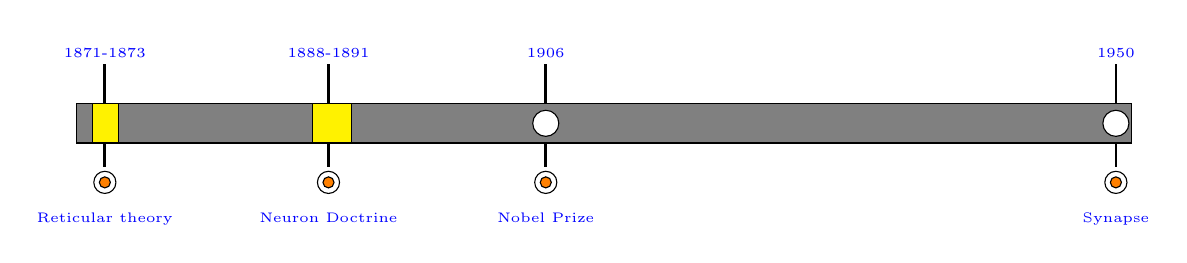
\begin{tikzpicture}[datemarker/.style={circle, draw=black,fill=white},textlabel/.style={anchor=center,text height=1.7ex,text depth=.25ex}] 
				\tikzset{every node/.style={font=\tiny, color=blue}}\draw[fill=gray](-0.2,0) rectangle (13.2,0.5) node[white, below]{}; 

				\onslide<1->{\draw[fill=yellow] (0,0) rectangle(0.329113924051, 0.5){};}
				\onslide<1->{\draw [line width=1pt] (0.16, 0.5) to (0.16, 1.0);} 
				\onslide<1->{\draw (0.16, 1.2) node [textlabel] {1871-1873 };}
				\onslide<1->{\draw [fill=orange](0.16, -0.5) circle (2pt){};}
				\onslide<1->{\draw (0.16, -0.5) circle (4pt){};}
				\onslide<1->{\draw [line width=1pt] (0.16, 0) to (0.16, -0.3);}
				\onslide<1->{\draw (0.16,-0.9) node [textlabel] {Reticular theory};}

				\onslide<3->{\draw[fill=yellow] (2.79746835443, 0) rectangle(3.29113924051, 0.5){};}
				\onslide<3->{\draw [line width=1pt] (3, 0.5) to (3, 1.0);} 
				\onslide<3->{\draw (3, 1.2) node [textlabel] {1888-1891 };}
				\onslide<3->{\draw [fill=orange](3, -0.5) circle (2pt){};}
				\onslide<3->{\draw (3, -0.5) circle (4pt){};}
				\onslide<3->{\draw [line width=1pt] (3, 0) to (3, -0.3);}
				\onslide<3->{\draw (3,-0.9) node [textlabel] {Neuron Doctrine};}

				\onslide<5->{\node at (5.75949367089, 0.25) [datemarker] {};}
				\onslide<5->{\draw [line width=1pt] (5.75949367089, 0.5) to (5.75949367089, 1.0);} 
				\onslide<5->{\draw (5.75949367089, 1.2) node [textlabel] {1906 };}
				\onslide<5->{\draw [fill=orange](5.75949367089, -0.5) circle (2pt){};}
				\onslide<5->{\draw (5.75949367089, -0.5) circle (4pt){};}
				\onslide<5->{\draw [line width=1pt] (5.75949367089, 0) to (5.75949367089, -0.3);}
				\onslide<5->{\draw (5.75949367089,-0.9) node [textlabel] {Nobel Prize};}

				\onslide<6->{\node at (13.0, 0.25) [datemarker] {};}
				\onslide<6->{\draw [line width=1pt] (13.0, 0.5) to (13.0, 1.0);} 
				\onslide<6->{\draw (13.0, 1.2) node [textlabel] {1950 };}
				\onslide<6->{\draw [fill=orange](13.0, -0.5) circle (2pt){};}
				\onslide<6->{\draw (13.0, -0.5) circle (4pt){};}
				\onslide<6->{\draw [line width=1pt] (13.0, 0) to (13.0, -0.3);}
				\onslide<6->{\draw (13.0,-0.9) node [textlabel] {Synapse};}
			\end{tikzpicture}
		\end{overlayarea}
	\end{minipage}
\end{frame}


\makeatother
%	\author{Mitesh M. Khapra}
	\title{Module 2}
	\subtitle{From Spring to Winter of AI}
		\author{}
		\institute{}
	\date{}
%\institute{Department of Computer Science and Engineering\\ Indian Institute of Technology Madras}
%\titlegraphic{
\includegraphics[height=1cm,width=2cm]{images/iitm_logo.png}}
%\titlegraphicii{\includegraphics[height=1cm,width=2cm]{logo2}}

\begin{frame}
	%\maketitle
	\myheading{Chapter 2: From Spring to Winter of AI}
\end{frame}

\begin{frame}
	\begin{minipage}[t][0.6\textheight][t]{\textwidth}
		\begin{columns}
			\column{0.5\textwidth}
				\begin{overlayarea}{\textwidth}{\textheight}
					\justify
					\only<1>{\myheading{McCulloch Pitts Neuron} McCulloch (neuroscientist) and Pitts (logician) proposed a highly simplified model of the neuron (1943)\cite{pitts}}
					\justify
					\only<2>{\myheading{Perceptron} ``the perceptron may eventually be able to learn, make decisions, and translate languages'' -Frank Rosenblatt}
					\justify
					\only<3>{\myheading{Perceptron} ``the embryo of an electronic computer that [the Navy] expects will be able to walk, talk, see, write, reproduce itself and be conscious of its existence.'' -New York Times}
					\justify
					\only<4>{\myheading{First generation Multilayer Perceptrons} Ivakhnenko et. al.\cite{mlp}}
					\justify
					\only<5>{\myheading{Perceptron Limitations} In their now famous book ``Perceptrons'', Minsky and Papert outlined the limits of what perceptrons could do \cite{perceptron}}
					\justify
					\only<6>{\myheading{AI Winter of connectionism} Almost lead to the abandonment of connectionist AI}
					\justify
					\only<7>{\myheading{Backpropagation} \begin{itemize} \item Discovered and rediscovered several times throughout 1960's and 1970's \item Werbos(1982) \cite{Werbos:81sensitivity} first used it in the context of artificial neural networks \item Eventually popularized by the work of Rumelhart et. al. in 1986\cite{Rumelhart:86}\end{itemize}}
					\justify
					\only<8>{\myheading{Gradient Descent} Cauchy discovered Gradient Descent motivated by the need to compute the orbit of heavenly bodies}
					\justify
					\only<9>{\myheading{Universal Approximation Theorem} A multilayered network of neurons with a single hidden layer can be used to approximate any continuous function to any desired precision\cite{hornik1989}}
				\end{overlayarea}
			\column{0.5\textwidth}
				\begin{overlayarea}{\textwidth}{\textheight}
					\begin{figure}
						\centering
						\only<1>{\includegraphics[scale=0.5]{"images/Artificial_Neuron/1943"}}
						\only<2>{\includegraphics[scale=0.4]{"images/Artificial_Neuron/1957"}}
						\only<3>{\includegraphics[scale=0.5]{"images/Artificial_Neuron/1958_1"}}
						\only<4>{\includegraphics[scale=0.25]{"images/Artificial_Neuron/1965-1968"}}
						\only<5>{\includegraphics[scale=0.25]{"images/Artificial_Neuron/1969"}}
						\only<7>{\includegraphics[scale=0.3]{"images/Artificial_Neuron/1986"}}
						\only<8>{\includegraphics[scale=0.2]{"images/Artificial_Neuron/1847"}}
						\only<9>{\includegraphics[scale=0.2]{"images/Artificial_Neuron/uat"}}
						%\only<10>{\includegraphics[scale=0.5]{"Artificial_Neuron/1989"}}
						%
					\end{figure}
				\end{overlayarea}
		\end{columns}
	\end{minipage}
	\begin{minipage}[t][0.4\textheight][t]{\textwidth}
		\begin{columns}
			\column{0.1\textwidth}
				\begin{overlayarea}{\textwidth}{\textheight}
					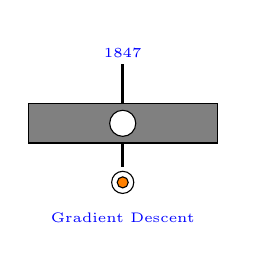
\begin{tikzpicture}[datemarker/.style={circle, draw=black,fill=white},textlabel/.style={anchor=center,text height=1.7ex,text depth=.25ex}]
					\tikzset{every node/.style={font=\tiny, color=blue}}\draw[fill=gray](-0.2,0) rectangle (2.2,0.5) node[white, below]{};
					\onslide<8->{\node at (1.0, 0.25) [datemarker] {};}
					\onslide<8->{\draw [line width=1pt] (1.0, 0.5) to (1.0, 1.0);}
					\onslide<8->{\draw (1.0, 1.2) node [textlabel] {1847 };}
					\onslide<8->{\draw [fill=orange](1.0, -0.5) circle (2pt){};}
					\onslide<8->{\draw (1.0, -0.5) circle (4pt){};}
					\onslide<8->{\draw [line width=1pt] (1.0, 0) to (1.0, -0.3);}
					\onslide<8->{\draw (1.0,-0.9) node [textlabel] {Gradient Descent};}
					\end{tikzpicture}
				\end{overlayarea}
			\column{0.9\textwidth}
				\begin{overlayarea}{\textwidth}{\textheight}
					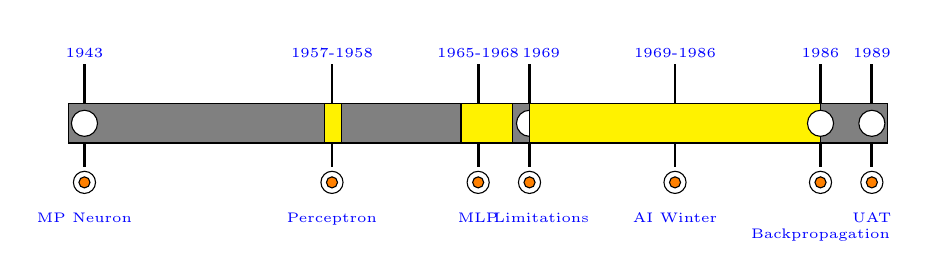
\begin{tikzpicture}[datemarker/.style={circle, draw=black,fill=white},textlabel/.style={anchor=center,text height=1.7ex,text depth=.25ex}] 
						\tikzset{every node/.style={font=\tiny, color=blue}}\draw[fill=gray](-0.2,0) rectangle (10.2,0.5) node[white, below]{}; 
						\onslide<1->{\node at (0.0, 0.25) [datemarker] {};}
						\onslide<1->{\draw [line width=1pt] (0.0, 0.5) to (0.0, 1.0);} 
						\onslide<1->{\draw (0.0, 1.2) node [textlabel] {1943 };}
						\onslide<1->{\draw [fill=orange](0.0, -0.5) circle (2pt){};}
						\onslide<1->{\draw (0.0, -0.5) circle (4pt){};}
						\onslide<1->{\draw [line width=1pt] (0.0, 0) to (0.0, -0.3);}
						\onslide<1->{\draw (0.0,-0.9) node [textlabel] {MP Neuron};}

						\onslide<2->{\draw[fill=yellow](3.04347826087, 0) rectangle (3.26086956522, 0.5){};}
						\onslide<2->{\draw [line width=1pt] (3.14347826087, 0.5) to (3.14347826087, 1.0);} 
						\onslide<2->{\draw (3.14347826087, 1.2) node [textlabel] {1957-1958 };}
						\onslide<2->{\draw [fill=orange](3.14347826087, -0.5) circle (2pt){};}
						\onslide<2->{\draw (3.14347826087, -0.5) circle (4pt){};}
						\onslide<2->{\draw [line width=1pt] (3.14347826087, 0) to (3.14347826087, -0.3);}
						\onslide<2->{\draw (3.14347826087,-0.9) node [textlabel] {Perceptron};}


						\onslide<4->{\draw[fill=yellow](4.78260869565, 0) rectangle (5.4347826087, 0.5){};}
						\onslide<4->{\draw [line width=1pt] (5.0, 0.5) to (5.0, 1.0);} 
						\onslide<4->{\draw (5.0, 1.2) node [textlabel] {1965-1968 };}
						\onslide<4->{\draw [fill=orange](5.0, -0.5) circle (2pt){};}
						\onslide<4->{\draw (5.0, -0.5) circle (4pt){};}
						\onslide<4->{\draw [line width=1pt] (5.0, 0) to (5.0, -0.3);}
						\onslide<4->{\draw (5.0,-0.9) node [textlabel] {MLP};}


						\onslide<5->{\node at (5.65217391304, 0.25) [datemarker] {};}
						\onslide<5->{\draw [line width=1pt] (5.65217391304, 0.5) to (5.65217391304, 1.0);} 
						\onslide<5->{\draw (5.80217391304, 1.2) node [textlabel] {1969 };}
						\onslide<5->{\draw [fill=orange](5.65217391304, -0.5) circle (2pt){};}
						\onslide<5->{\draw (5.65217391304, -0.5) circle (4pt){};}
						\onslide<5->{\draw [line width=1pt] (5.65217391304, 0) to (5.65217391304, -0.3);}
						\onslide<5->{\draw (5.80217391304,-0.9) node [textlabel] {Limitations};}

						\onslide<6->{\draw[fill=yellow](5.65217391304, 0) rectangle (9.34782608696, 0.5){};}
						\onslide<6->{\draw [line width=1pt] (7.5, 0.5) to (7.5, 1.0);} 
						\onslide<6->{\draw (7.5, 1.2) node [textlabel] {1969-1986};}
						\onslide<6->{\draw [fill=orange](7.5, -0.5) circle (2pt){};}
						\onslide<6->{\draw (7.5, -0.5) circle (4pt){};}
						\onslide<6->{\draw [line width=1pt] (7.5, 0) to (7.5, -0.3);}
						\onslide<6->{\draw (7.5,-0.9) node [textlabel] {AI Winter};}

						\onslide<7->{\node at (9.34782608696, 0.25) [datemarker] {};}
						\onslide<7->{\draw [line width=1pt] (9.34782608696, 0.5) to (9.34782608696, 1.0);} 
						\onslide<7->{\draw (9.34782608696, 1.2) node [textlabel] {1986 };}
						\onslide<7->{\draw [fill=orange](9.34782608696, -0.5) circle (2pt){};}
						\onslide<7->{\draw (9.34782608696, -0.5) circle (4pt){};}
						\onslide<7->{\draw [line width=1pt] (9.34782608696, 0) to (9.34782608696, -0.3);}
						\onslide<7->{\draw (9.34782608696,-1.1) node [textlabel] {Backpropagation};}

						\onslide<9->{\node at (10.0, 0.25) [datemarker] {};}
						\onslide<9->{\draw [line width=1pt] (10.0, 0.5) to (10.0, 1.0);} 
						\onslide<9->{\draw (10.0, 1.2) node [textlabel] {1989 };}
						\onslide<9->{\draw [fill=orange](10.0, -0.5) circle (2pt){};}
						\onslide<9->{\draw (10.0, -0.5) circle (4pt){};}
						\onslide<9->{\draw [line width=1pt] (10.0, 0) to (10.0, -0.3);}
						\onslide<9->{\draw (10.0,-0.9) node [textlabel] {UAT};}
					\end{tikzpicture}
				\end{overlayarea}
		\end{columns}
	\end{minipage}
\end{frame}


\makeatother
%	\author{Mitesh M. Khapra}
	\title{Module 3}
	\subtitle{The Deep Revival}
		\author{}
		\institute{}
	\date{}
%\institute{Department of Computer Science and Engineering\\ Indian Institute of Technology Madras}
%\titlegraphic{
\includegraphics[height=1cm,width=2cm]{images/iitm_logo.png}}
%\titlegraphicii{\includegraphics[height=1cm,width=2cm]{logo2}}

\begin{frame}
	\myheading{Chapter 3: The Deep Revival}
\end{frame}

\begin{frame}
	\begin{minipage}[t][0.6\textheight][t]{\textwidth}
		\begin{columns}
			\column{0.5\textwidth}
				\begin{overlayarea}{\textwidth}{\textheight}
					\justify
					\only<1>{\myheading{Unsupervised Pre-Training}}
					\only<1>{Hinton and  Salakhutdinov described an effective way of initializing the weights that allows deep autoencoder networks to learn a low-dimensional representation of data. \cite{Salakhutdinov:2012:ELP:2330716.2330717}}
				\end{overlayarea}
			\column{0.5\textwidth}
					\begin{overlayarea}{\textwidth}{\textheight}
						\begin{figure}
							\centering
							\only<1>{\includegraphics[scale=0.7]{"images/Renewed_Interest/2006_1"}
						\end{figure}
					\end{overlayarea}
		\end{columns}
	\end{minipage}
	\begin{minipage}[t][0.4\textheight][t]{\textwidth}
		\begin{columns}
		\column{0.1\textwidth}
		\column{0.9\textwidth}
			\begin{overlayarea}{\textwidth}{\textheight}
			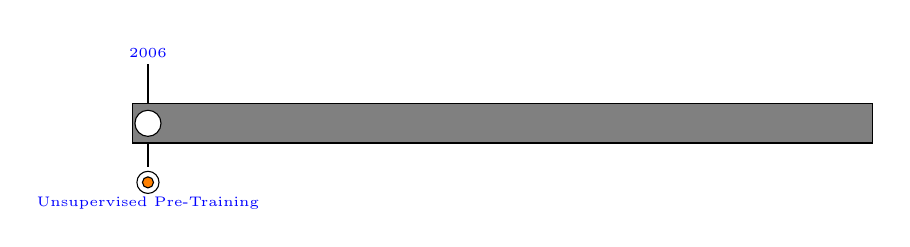
\begin{tikzpicture}[datemarker/.style={circle, draw=black,fill=white},textlabel/.style={anchor=center,text height=1.7ex,text depth=.25ex}] 
			\tikzset{every node/.style={font=\tiny, color=blue}}\draw[fill=gray](-0.2,0) rectangle (9.2,0.5) node[white, below]{}; 
			\onslide<1>{\node at (0.0, 0.25) [datemarker] {};}
			\onslide<1>{\draw [line width=1pt] (0.0, 0.5) to (0.0, 1.0);} 
			\onslide<1>{\draw (0.0, 1.2) node [textlabel] {2006 };}
			\onslide<1>{\draw [fill=orange](0.0, -0.5) circle (2pt){};}
			\onslide<1>{\draw (0.0, -0.5) circle (4pt){};}
			\onslide<1>{\draw [line width=1pt] (0.0, 0) to (0.0, -0.3);}
			\onslide<1>{\draw (0.0,-0.7) node [textlabel] {Unsupervised Pre-Training};}
			\end{tikzpicture}
			\end{overlayarea}
		\end{columns}
	\end{minipage}
\end{frame}
\begin{frame}
\begin{minipage}[t][0.6\textheight][t]{\textwidth}
\begin{columns}
\column{0.5\textwidth}
\begin{overlayarea}{\textwidth}{\textheight}
\justify
\only<1>{\myheading{Unsupervised Pre-Training}}
\only<1>{The idea of unsupervised pre-training actually dates back to 1991-1993 (J. Schmidhuber) when it was used to train a ``Very Deep Learner''}
\only<2>{\myheading{More insights (2007-2009)}}
\only<2>{Further Investigations into the effectiveness of Unsupervised Pre-training}

\only<3>{\myheading{Success in Handwriting Recognition}}
\only<4>{\myheading{Success in Speech Recognition}}
\only<5>{\myheading{ New record on MNIST }}
\only<6>{\myheading{ First Superhuman Visual Pattern Recognition}}
\only<7->{\myheading{Winning more visual recognition challenges}}

\only<3>{Graves et. al. outperformed all entries in an international Arabic recognition competition \cite{NIPS2008_3449}}
\only<4>{Dahl et. al. showed relative error reduction of 16.0\% and 23.2\% over a state of the art system \cite{Dahl:2012:CPD:2335874.2336015}}
\only<5>{Ciresan et. al. set a new record on the MNIST dataset using good old backpropagation on GPUs (GPUs enter the scene)\cite{DBLP:journals/corr/abs-1003-0358}}
\only<6>{D. C. Ciresan et. al. achieved 0.56\% error rate in the IJCNN Traffic Sign Recognition Competition \cite{DBLP:journals/corr/abs-1202-2745}}
\only<7->{\begin{table}
\begin{tabular}{ccc}
\textbf{Network}&\textbf{Error}&\textbf{Layers}\\
\onslide<7->{AlexNet \cite{NIPS2012_4824}}&\onslide<7->{16.0\%}&\onslide<7->{8}\\
\onslide<8->{ZFNet \cite{DBLP:journals/corr/ZeilerF13}}&\onslide<8->{11.2\%}&\onslide<8->{8}\\
\onslide<9->{VGGNet \cite{DBLP:journals/corr/SimonyanZ14a}}&\onslide<9->{7.3\%}&\onslide<9->{19}\\
\onslide<10->{GoogLeNet \cite{DBLP:journals/corr/SzegedyLJSRAEVR14}}&\onslide<10->{6.7\%}&\onslide<10->{22}\\
\onslide<11->{MS ResNet \cite{DBLP:journals/corr/HeZRS15}}&\onslide<11->{3.6\%}&\onslide<11->{152!!}\\
\end{tabular}
\end{table}
}




\end{overlayarea}
\column{0.5\textwidth}
\begin{overlayarea}{\textwidth}{\textheight}
\begin{figure}
\centering
\only<1>{\includegraphics[scale=0.7]{"images/Renewed_Interest/2006_1"}}
\only<2>{\includegraphics[scale=0.23]{"images/Renewed_Interest/2007"}}
\only<3>{\includegraphics[scale=0.15]{"images/Renewed_Interest/2009"}}
\only<4>{\includegraphics[scale=0.5]{"images/Renewed_Interest/2010_1"}}
\only<5>{\includegraphics[scale=0.5]{"images/Renewed_Interest/2010"}}
\only<6>{\includegraphics[scale=0.4]{"images/Renewed_Interest/2011"}}
\only<7->{\includegraphics[scale=0.4]{"images/Renewed_Interest/2012_1"}}


\end{figure}
\end{overlayarea}
\end{columns}
\end{minipage}
\begin{minipage}[t][0.4\textheight][t]{\textwidth}
\begin{columns}
\column{0.1\textwidth}
\begin{overlayarea}{\textwidth}{\textheight}
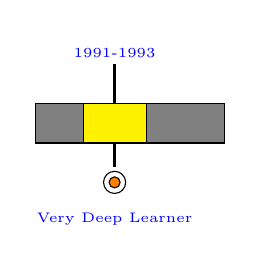
\begin{tikzpicture}[datemarker/.style={circle, draw=black,fill=white},textlabel/.style={anchor=center,text height=1.7ex,text depth=.25ex}]
\tikzset{every node/.style={font=\tiny, color=blue}}\draw[fill=gray](-0.2,0) rectangle (2.2,0.5) node[white, below]{};
%\onslide<1->{\node at (0.0, 0.25) [datemarker] {};}
%\onslide<1->{\draw [line width=1pt] (0.0, 0.5) to (0.0, 1.0);}
%\onslide<1->{\draw (0.0, 1.2) node [textlabel] {1990 };}
%\onslide<1->{\draw [fill=orange](0.0, -0.5) circle (2pt){};}
%\onslide<1->{\draw (0.0, -0.5) circle (4pt){};}
%\onslide<1->{\draw [line width=1pt] (0.0, 0) to (0.0, -0.3);}
%\onslide<1->{\draw (0.0,-0.9) node [textlabel] {};}
\onslide<1->{\draw[fill=yellow] (0.4, 0) rectangle (1.2, 0.5){};}
%\onslide<2->{\node at (0.4, 0.25) [datemarker] {};}
\onslide<1->{\draw [line width=1pt] (0.8, 0.5) to (0.8, 1.0);}
\onslide<1->{\draw (0.8, 1.2) node [textlabel] {1991-1993 };}
\onslide<1->{\draw [fill=orange](0.8, -0.5) circle (2pt){};}
\onslide<1->{\draw (0.8, -0.5) circle (4pt){};}
\onslide<1->{\draw [line width=1pt] (0.8, 0) to (0.8, -0.3);}
\onslide<1->{\draw (0.8,-0.9) node [textlabel] {Very Deep Learner};}
\end{tikzpicture}
\end{overlayarea}


\column{0.9\textwidth}
\begin{overlayarea}{\textwidth}{\textheight}
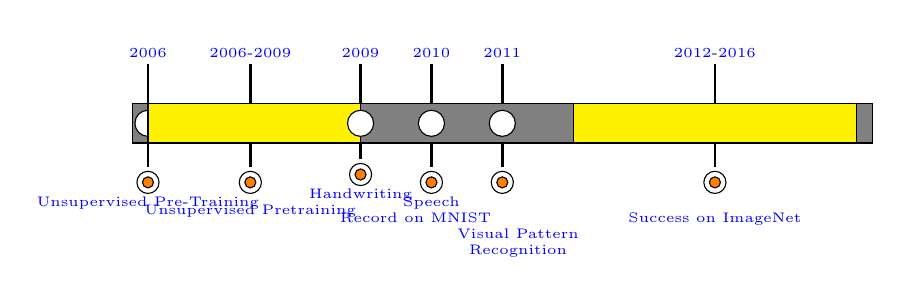
\begin{tikzpicture}[datemarker/.style={circle, draw=black,fill=white},textlabel/.style={anchor=center,text height=1.7ex,text depth=.25ex}] 
\tikzset{every node/.style={font=\tiny, color=blue}}\draw[fill=gray](-0.2,0) rectangle (9.2,0.5) node[white, below]{}; 
\onslide<1>{\node at (0.0, 0.25) [datemarker] {};}
\onslide<1>{\draw [line width=1pt] (0.0, 0.5) to (0.0, 1.0);} 
\onslide<1>{\draw (0.0, 1.2) node [textlabel] {2006 };}
\onslide<1>{\draw [fill=orange](0.0, -0.5) circle (2pt){};}
\onslide<1>{\draw (0.0, -0.5) circle (4pt){};}
\onslide<1>{\draw [line width=1pt] (0.0, 0) to (0.0, -0.3);}
\onslide<1>{\draw (0.0,-0.7) node [textlabel] {Unsupervised Pre-Training};}

\onslide<2->{\draw [fill=yellow] (0,0) rectangle (2.7, 0.5){};}
\onslide<2->{\draw [line width=1pt] (1.3, 0.5) to (1.3, 1.0);} 
\onslide<2->{\draw (1.3, 1.2) node [textlabel] {2006-2009};}
\onslide<2->{\draw [fill=orange](1.3, -0.5) circle (2pt){};}
\onslide<2->{\draw (1.3, -0.5) circle (4pt){};}
\onslide<2->{\draw [line width=1pt] (1.3, 0) to (1.3, -0.3);}
\onslide<2->{\draw (1.3,-0.8) node [textlabel] {Unsupervised Pretraining};}


\onslide<3->{\node at (2.7, 0.25) [datemarker] {};}
\onslide<3->{\draw [line width=1pt] (2.7, 0.5) to (2.7, 1.0);} 
\onslide<3->{\draw (2.7, 1.2) node [textlabel] {2009 };}
\onslide<3->{\draw [fill=orange](2.7, -0.4) circle (2pt){};}
\onslide<3->{\draw (2.7, -0.4) circle (4pt){};}
\onslide<3->{\draw [line width=1pt] (2.7, 0) to (2.7, -0.2);}
\onslide<3->{\draw (2.7,-0.6) node [textlabel] {Handwriting};}

\onslide<4->{\node at (3.6, 0.25) [datemarker] {};}
\onslide<4->{\draw [line width=1pt] (3.6, 0.5) to (3.6, 1.0);} 
\onslide<4->{\draw (3.6, 1.2) node [textlabel] {2010 };}
\onslide<4->{\draw [fill=orange](3.6, -0.5) circle (2pt){};}
\onslide<4->{\draw (3.6, -0.5) circle (4pt){};}
\onslide<4->{\draw [line width=1pt] (3.6, 0) to (3.6, -0.3);}
\onslide<4->{\draw (3.6,-0.7) node [textlabel] {Speech};}
\onslide<5->{\draw (3.4,-0.9) node [textlabel] {Record on MNIST};}



\onslide<6->{\node at (4.5, 0.25) [datemarker] {};}
\onslide<6->{\draw [line width=1pt] (4.5, 0.5) to (4.5, 1.0);} 
\onslide<6->{\draw (4.5, 1.2) node [textlabel] {2011 };}
\onslide<6->{\draw [fill=orange](4.5, -0.5) circle (2pt){};}
\onslide<6->{\draw (4.5, -0.5) circle (4pt){};}
\onslide<6->{\draw [line width=1pt] (4.5, 0) to (4.5, -0.3);}
\onslide<6->{\draw (4.7,-1.1) node [textlabel] {Visual Pattern};}
\onslide<6->{\draw (4.7,-1.3) node [textlabel] {Recognition};}


\onslide<7->{\draw [fill=yellow] (5.4,0) rectangle (9.0, 0.5){};}
\onslide<7->{\draw [line width=1pt] (7.2, 0.5) to (7.2, 1.0);} 
\onslide<7->{\draw (7.2, 1.2) node [textlabel] {2012-2016 };}
\onslide<7->{\draw [fill=orange](7.2, -0.5) circle (2pt){};}
\onslide<7->{\draw (7.2, -0.5) circle (4pt){};}
\onslide<7->{\draw [line width=1pt] (7.2, 0) to (7.2, -0.3);}
\onslide<7->{\draw (7.2,-0.9) node [textlabel] {Success on ImageNet};}
\end{tikzpicture}
\end{overlayarea}
\end{columns}
\end{minipage}
\end{frame}

	\makeatother
%	\author{Mitesh M. Khapra}
	\title{Module 4}
	\subtitle{Cats}
		\author{}
		\institute{}
	\date{}
%\institute{Department of Computer Science and Engineering\\ Indian Institute of Technology Madras}
%\titlegraphic{
\includegraphics[height=1cm,width=2cm]{images/iitm_logo.png}}
%\titlegraphicii{\includegraphics[height=1cm,width=2cm]{logo2}}

\begin{frame}
	\maketitle
\end{frame}

\begin{frame}
\begin{minipage}[t][0.6\textheight][t]{\textwidth}
\begin{columns}
\column{0.5\textwidth}
\begin{overlayarea}{\textwidth}{\textheight}
\justify
\only<1>{\myheading{Hubel and Wiesel Experiment} Experimentally showed that each neuron has a fixed receptive field - i.e. a neuron will fire only in response to a visual stimuli in a specific region in the visual space \cite{wiesel:1959}}
\only<2>{\myheading{Neocognitron} Used for Handwritten character recognition and pattern recognition (Fukushima et. al.) \cite{fukushima:1980}}
\only<3>{\myheading{Convolutional Neural Network} Handwriting digit recognition using backpropagation over a Convolutional Neural Network (LeCun et. al.) \cite{LeCun:89}}
\only<4>{\myheading{LeNet-5} Introduced the (now famous) MNIST dataset (LeCun et. al.)\cite{LeCun:98}}
\end{overlayarea}
\column{0.5\textwidth}
\begin{overlayarea}{\textwidth}{\textheight}
\begin{figure}
\centering
\only<1>{\includegraphics[scale=0.3]{"images/Renewed_Interest/CNN_History/1959"}}
\only<2>{\includegraphics[scale=0.5]{"images/Renewed_Interest/CNN_History/1980"}}
\only<3>{\includegraphics[scale=0.5]{"images/Renewed_Interest/CNN_History/1989"}}
\only<4>{\includegraphics[scale=0.5]{"images/Renewed_Interest/CNN_History/1998"}}
\end{figure}
\end{overlayarea}
\end{columns}
\end{minipage}
\begin{minipage}[t][0.4\textheight][t]{\textwidth}
\begin{overlayarea}{\textwidth}{\textheight}
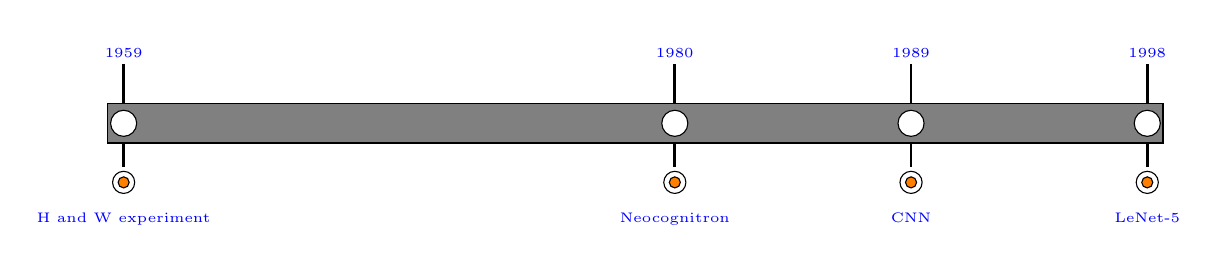
\begin{tikzpicture}[datemarker/.style={circle, draw=black,fill=white},textlabel/.style={anchor=center,text height=1.7ex,text depth=.25ex}] 
\tikzset{every node/.style={font=\tiny, color=blue}}\draw[fill=gray](-0.2,0) rectangle (13.2,0.5) node[white, below]{}; 
\onslide<1->{\node at (0.0, 0.25) [datemarker] {};}
\onslide<1->{\draw [line width=1pt] (0.0, 0.5) to (0.0, 1.0);} 
\onslide<1->{\draw (0.0, 1.2) node [textlabel] {1959 };}
\onslide<1->{\draw [fill=orange](0.0, -0.5) circle (2pt){};}
\onslide<1->{\draw (0.0, -0.5) circle (4pt){};}
\onslide<1->{\draw [line width=1pt] (0.0, 0) to (0.0, -0.3);}
\onslide<1->{\draw (0.0,-0.9) node [textlabel] {H and W experiment};}

\onslide<2->{\node at (7.0, 0.25) [datemarker] {};}
\onslide<2->{\draw [line width=1pt] (7.0, 0.5) to (7.0, 1.0);} 
\onslide<2->{\draw (7.0, 1.2) node [textlabel] {1980 };}
\onslide<2->{\draw [fill=orange](7.0, -0.5) circle (2pt){};}
\onslide<2->{\draw (7.0, -0.5) circle (4pt){};}
\onslide<2->{\draw [line width=1pt] (7.0, 0) to (7.0, -0.3);}
\onslide<2->{\draw (7.0,-0.9) node [textlabel] {Neocognitron};}

\onslide<3->{\node at (10.0, 0.25) [datemarker] {};}
\onslide<3->{\draw [line width=1pt] (10.0, 0.5) to (10.0, 1.0);} 
\onslide<3->{\draw (10.0, 1.2) node [textlabel] {1989 };}
\onslide<3->{\draw [fill=orange](10.0, -0.5) circle (2pt){};}
\onslide<3->{\draw (10.0, -0.5) circle (4pt){};}
\onslide<3->{\draw [line width=1pt] (10.0, 0) to (10.0, -0.3);}
\onslide<3->{\draw (10.0,-0.9) node [textlabel] {CNN};}

\onslide<4->{\node at (13.0, 0.25) [datemarker] {};}
\onslide<4->{\draw [line width=1pt] (13.0, 0.5) to (13.0, 1.0);} 
\onslide<4->{\draw (13.0, 1.2) node [textlabel] {1998 };}
\onslide<4->{\draw [fill=orange](13.0, -0.5) circle (2pt){};}
\onslide<4->{\draw (13.0, -0.5) circle (4pt){};}
\onslide<4->{\draw [line width=1pt] (13.0, 0) to (13.0, -0.3);}
\onslide<4->{\draw (13.0,-0.9) node [textlabel] {LeNet-5};}
\end{tikzpicture}
\end{overlayarea}
\end{minipage}
\end{frame}

\begin{frame}
    \myheading{An algorithm inspired by an experiment on cats is today used to detect cats in videos :-)}
\end{frame}

\makeatother
%	\author{Mitesh M. Khapra}
	\title{Module 5}
	\subtitle{Faster, Higher, Stronger}
		\author{}
		\institute{}
	\date{}
%\institute{Department of Computer Science and Engineering\\ Indian Institute of Technology Madras}
%\titlegraphic{
\includegraphics[height=1cm,width=2cm]{images/iitm_logo.png}}
%\titlegraphicii{\includegraphics[height=1cm,width=2cm]{logo2}}

\begin{frame}
	\myheading{Chapter 5: Faster, higher, stronger}
\end{frame}

\begin{frame}
\begin{minipage}[t][0.6\textheight][t]{\textwidth}
\begin{columns}


\column{0.5\textwidth}
\begin{overlayarea}{\textwidth}{\textheight}
\justify
\only<1->{\myheading{Better Optimization Methods} Faster convergence, better accuracies}
\end{overlayarea}
\column{0.5\textwidth}
\begin{overlayarea}{\textwidth}{\textheight}
\begin{figure}
\centering
\only<1->{\includegraphics[scale=0.3]{"images/sgd_quiver84"}}
\end{figure}
\end{overlayarea}

\end{columns}
\end{minipage}

\begin{minipage}[t][0.5\textheight][t]{\textwidth}
\begin{overlayarea}{\textwidth}{\textheight}
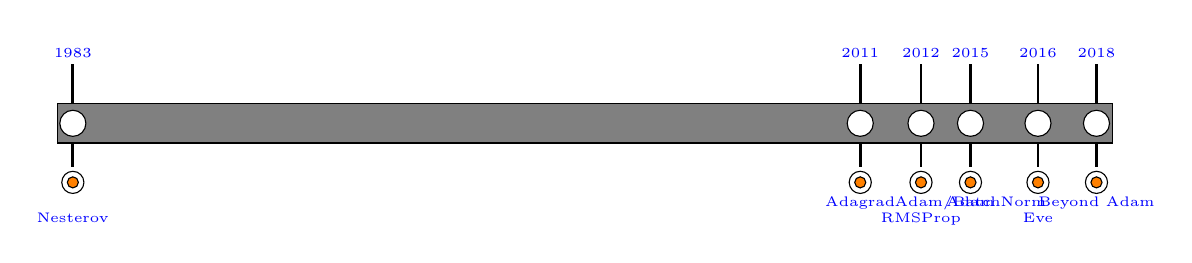
\begin{tikzpicture}[datemarker/.style={circle, draw=black,fill=white},textlabel/.style={anchor=center,text height=1.7ex,text depth=.25ex}]
\tikzset{every node/.style={font=\tiny, color=blue}}\draw[fill=gray](-0.2,0) rectangle (13.2,0.5) node[white, below]{};
\onslide<1->{\node at (0.0, 0.25) [datemarker] {};}
\onslide<1->{\draw [line width=1pt] (0.0, 0.5) to (0.0, 1.0);}
\onslide<1->{\draw (0.0, 1.2) node [textlabel]{1983};}
\onslide<1->{\draw [fill=orange](0.0, -0.5) circle (2pt){};}
\onslide<1->{\draw(0.0, -0.5) circle (4pt){};}
\onslide<1->{\draw [line width=1pt] (0.0, 0) to (0.0, -0.3);}
\onslide<1->{\draw (0.0,-0.9) node [textlabel] {Nesterov};}

\onslide<2->{\node at (10.0, 0.25) [datemarker] {};}
\onslide<2->{\draw [line width=1pt] (10.0, 0.5) to (10.0, 1.0);}
\onslide<2->{\draw (10.0, 1.2) node [textlabel]{2011};}
\onslide<2->{\draw [fill=orange](10.0, -0.5) circle (2pt){};}
\onslide<2->{\draw(10.0, -0.5) circle (4pt){};}
\onslide<2->{\draw [line width=1pt] (10.0, 0) to (10.0, -0.3);}
\onslide<2->{\draw (10.0,-0.7) node [textlabel] {Adagrad};}

\onslide<3->{\node at (10.7714285714, 0.25) [datemarker] {};}
\onslide<3->{\draw [line width=1pt] (10.7714285714, 0.5) to (10.7714285714, 1.0);}
\onslide<3->{\draw (10.7714285714, 1.2) node [textlabel]{2012};}
\onslide<3->{\draw [fill=orange](10.7714285714, -0.5) circle (2pt){};}
\onslide<3->{\draw(10.7714285714, -0.5) circle (4pt){};}
\onslide<3->{\draw [line width=1pt] (10.7714285714, 0) to (10.7714285714, -0.3);}
\onslide<3->{\draw (10.7714285714,-0.9) node [textlabel] {RMSProp};}

\onslide<4->{\node at (11.4, 0.25) [datemarker] {};}
\onslide<4->{\draw [line width=1pt] (11.4, 0.5) to (11.4, 1.0);}
\onslide<4->{\draw (11.4, 1.2) node [textlabel]{2015};}
\onslide<4->{\draw [fill=orange](11.4, -0.5) circle (2pt){};}
\onslide<4->{\draw(11.4, -0.5) circle (4pt){};}
\onslide<4->{\draw [line width=1pt] (11.4, 0) to (11.4, -0.3);}
\onslide<4-6>{\draw (11.4,-0.7) node [textlabel] {Adam};}

\onslide<5->{\node at (12.2571428571, 0.25) [datemarker] {};}
\onslide<5->{\draw [line width=1pt] (12.2571428571, 0.5) to (12.2571428571, 1.0);}
\onslide<5->{\draw (12.2571428571, 1.2) node [textlabel]{2016};}
\onslide<5->{\draw [fill=orange](12.2571428571, -0.5) circle (2pt){};}
\onslide<5->{\draw(12.2571428571, -0.5) circle (4pt){};}
\onslide<5->{\draw [line width=1pt] (12.2571428571, 0) to (12.2571428571, -0.3);}
\onslide<5->{\draw (12.2571428571,-0.9) node [textlabel] {Eve};}
\onslide<6->{\node at (13.0, 0.25) [datemarker] {};}
\onslide<6->{\draw [line width=1pt] (13.0, 0.5) to (13.0, 1.0);}
\onslide<6->{\draw (13.0, 1.2) node [textlabel]{2018};}
\onslide<6->{\draw [fill=orange](13.0, -0.5) circle (2pt){};}
\onslide<6->{\draw(13.0, -0.5) circle (4pt){};}
\onslide<6->{\draw [line width=1pt] (13.0, 0) to (13.0, -0.3);}
\onslide<6->{\draw (13.0,-0.7) node [textlabel] {Beyond Adam};}

\onslide<7->{\draw (11.4,-0.7) node [textlabel] {Adam/BatchNorm};}
\end{tikzpicture}
\end{overlayarea}
\end{minipage}
\end{frame}


\begin{frame}
\begin{minipage}[t][0.6\textheight][t]{\textwidth}
\begin{columns}
\column{0.5\textwidth}
\begin{overlayarea}{\textwidth}{\textheight}
\only<1->{\myheading{Better Activation Functions}}
\justify
\only<1>{The \textbf{logistic function} was the most popular choice in the 80's }
\only<2>{The \textbf{tanh function} which is zero centered leads to better convergence
\cite{LeCun:91}}
\only<3->{ More recently it has been shown that \textbf{Rectified Linear Units (ReLUs)} and their variants lead to better performance \cite{Nair2010}, \cite{Krizhevsky:2012},\cite{Maas2013}}
\end{overlayarea}
\column{0.5\textwidth}
\begin{overlayarea}{\textwidth}{\textheight}
\begin{figure}
\centering
\only<1>{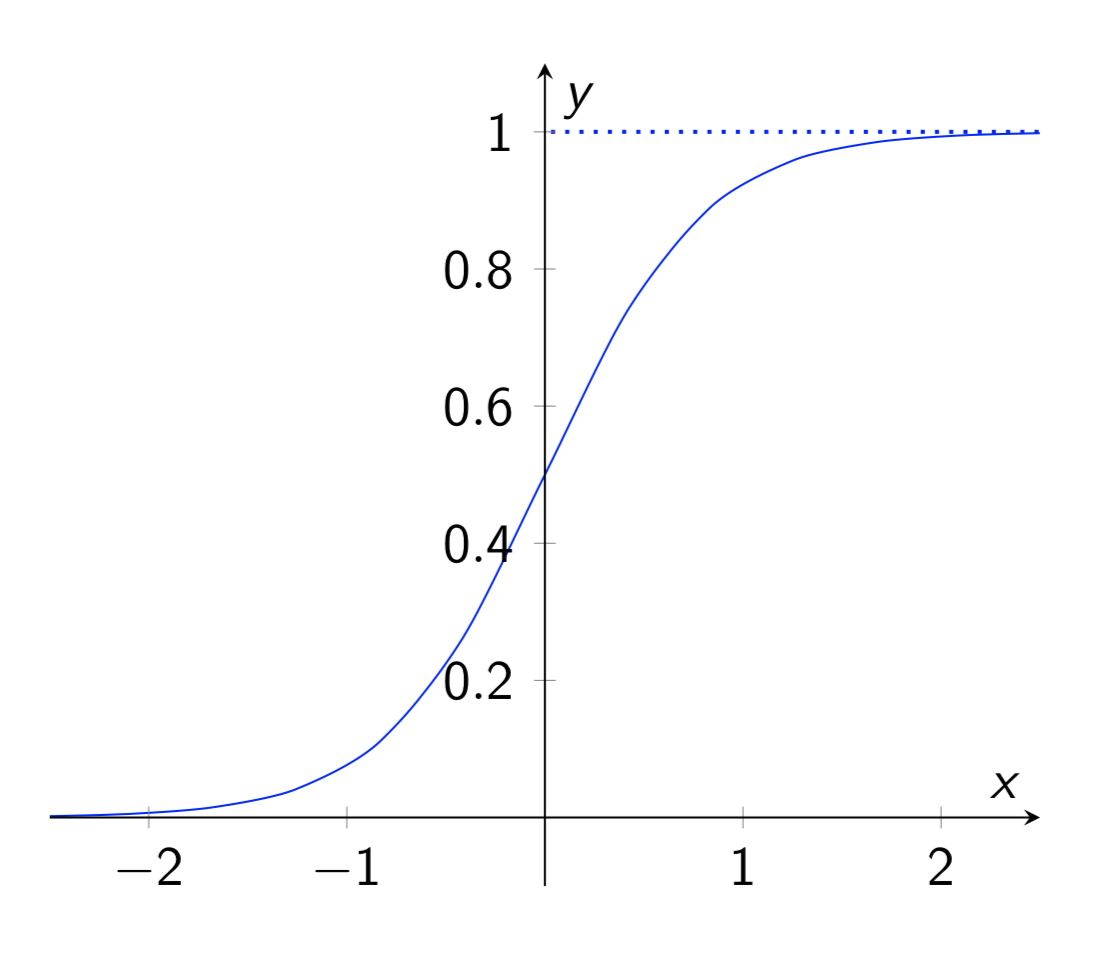
\includegraphics[scale=0.2]{images/logistic}}
\only<2>{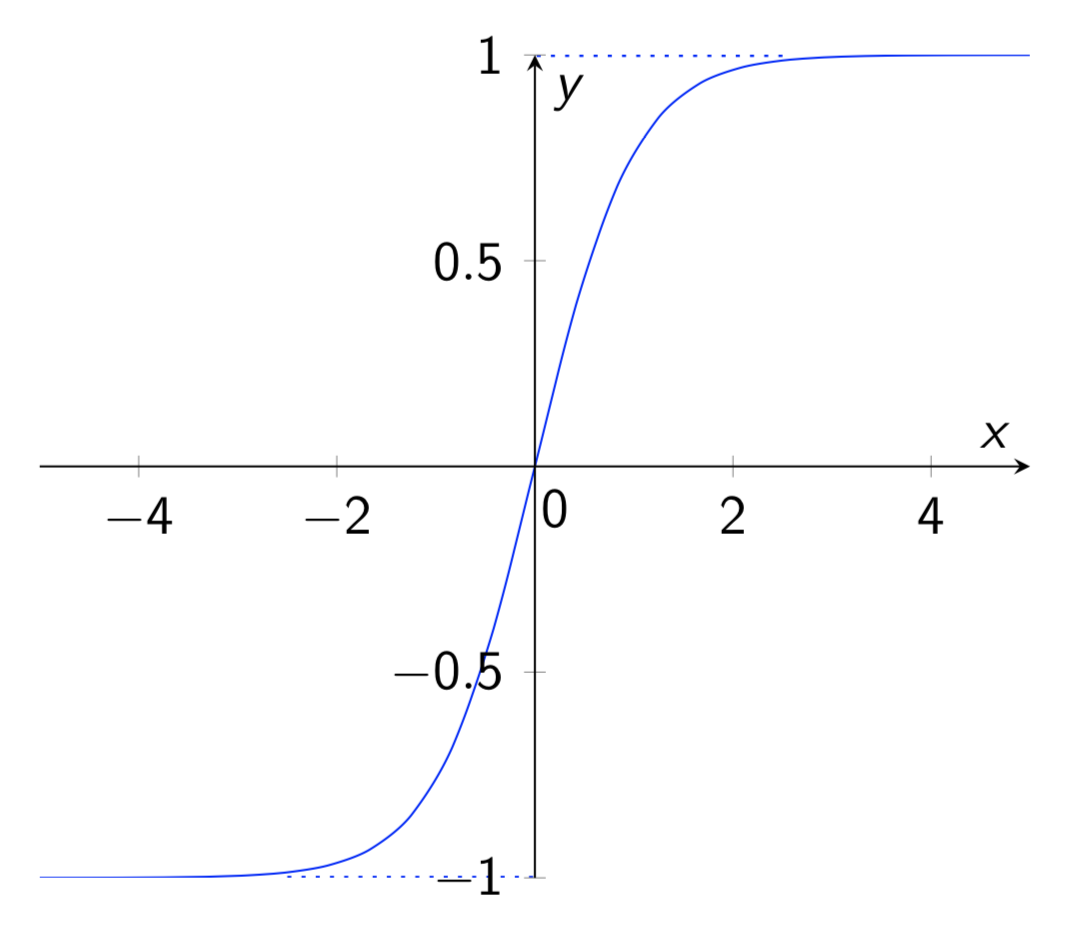
\includegraphics[scale=0.2]{images/tanh}}
%\only<3>{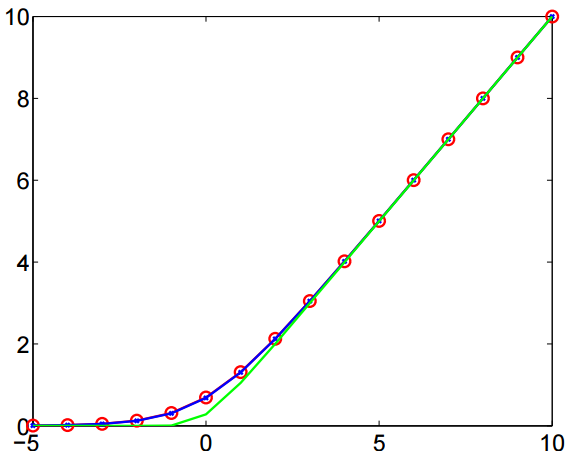
\includegraphics[scale=0.2]{images/relu_rbm}}
%\only<4>{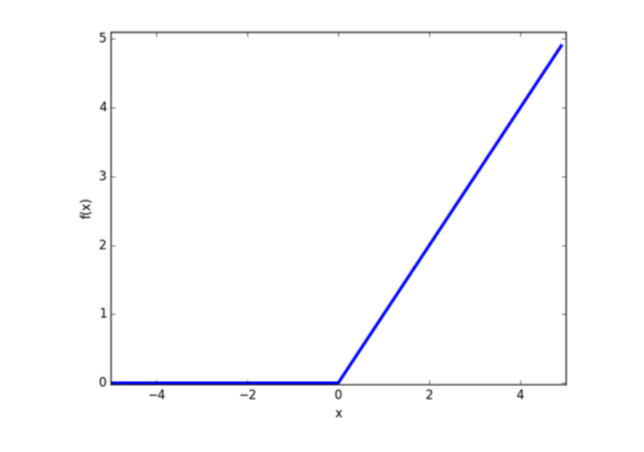
\includegraphics[scale=0.5]{images/relu_cnn}}
\only<3->{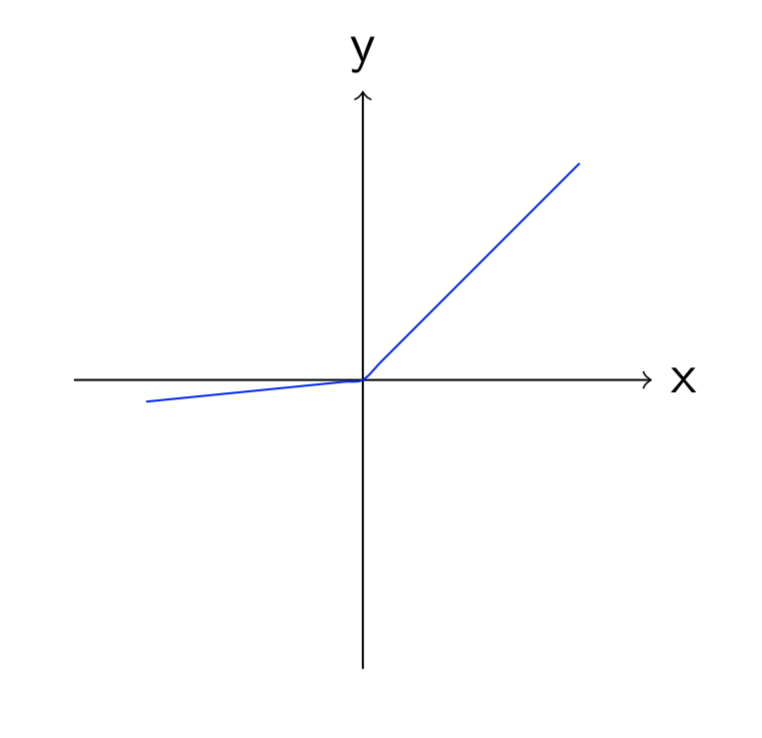
\includegraphics[scale=0.4]{images/leaky_relu}}
%\only<6>{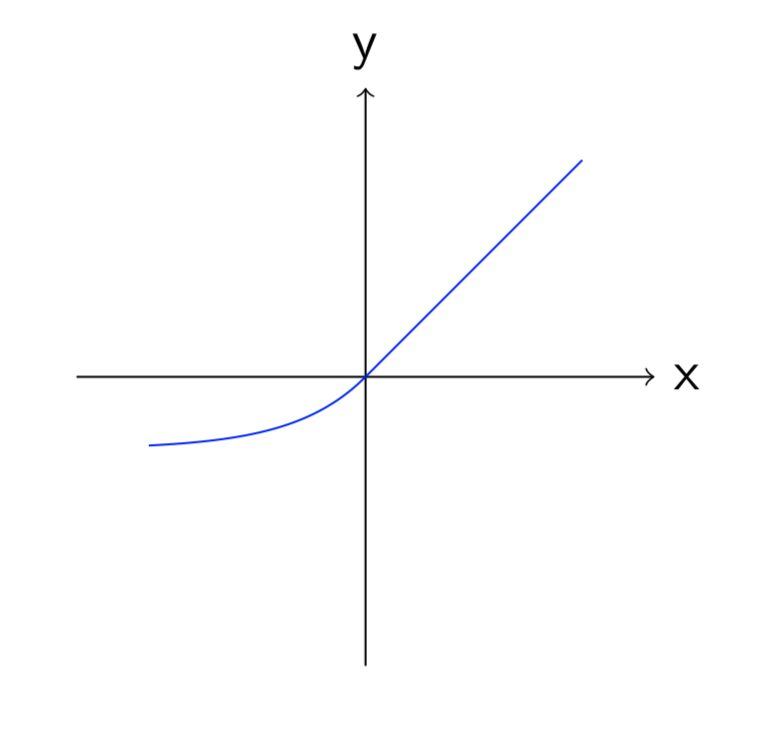
\includegraphics[scale=0.4]{images/exponential_relu}}
%\only<7>{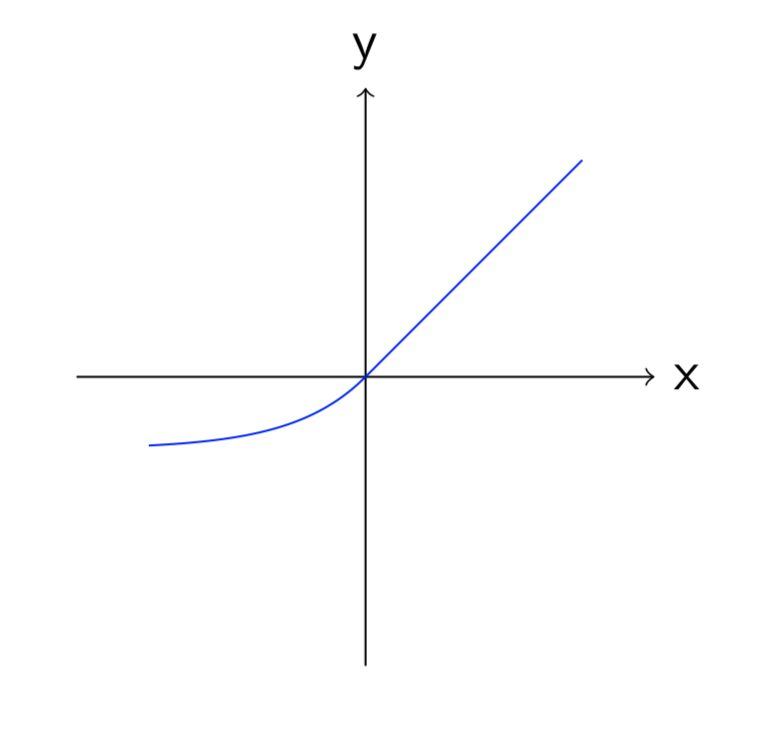
\includegraphics[scale=0.4]{images/exponential_relu}}
\end{figure}
\end{overlayarea}
\end{columns}
\end{minipage}
\begin{minipage}[t][0.4\textheight][t]{\textwidth}
\begin{overlayarea}{\textwidth}{\textheight}
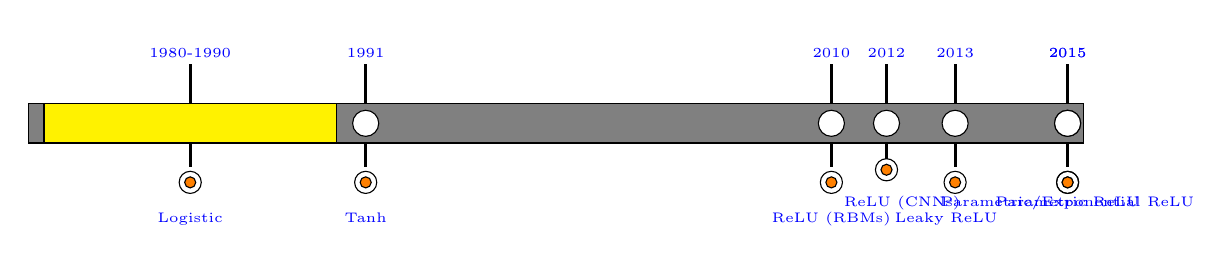
\begin{tikzpicture}[datemarker/.style={circle, draw=black,fill=white},textlabel/.style={anchor=center,text height=1.7ex,text depth=.25ex}]
\tikzset{every node/.style={font=\tiny, color=blue}}\draw[fill=gray](-0.2,0) rectangle (13.2,0.5) node[white, below]{};
\onslide<1->{\draw[fill=yellow](0.0,0) rectangle (3.71428571429, 0.5){};}
\onslide<1->{\draw [line width=1pt] (1.85714285714, 0.5) to (1.85714285714, 1.0);}
\onslide<1->{\draw (1.85714285714, 1.2) node [textlabel]{1980-1990};}
\onslide<1->{\draw [fill=orange](1.85714285714, -0.5) circle (2pt){};}
\onslide<1->{\draw(1.85714285714, -0.5) circle (4pt){};}
\onslide<1->{\draw [line width=1pt] (1.85714285714, 0) to (1.85714285714, -0.3);}
\onslide<1->{\draw (1.85714285714,-0.9) node [textlabel] {Logistic};}
\onslide<2->{\node at (4.08571428571, 0.25) [datemarker] {};}
\onslide<2->{\draw [line width=1pt] (4.08571428571, 0.5) to (4.08571428571, 1.0);}
\onslide<2->{\draw (4.08571428571, 1.2) node [textlabel]{1991};}
\onslide<2->{\draw [fill=orange](4.08571428571, -0.5) circle (2pt){};}
\onslide<2->{\draw(4.08571428571, -0.5) circle (4pt){};}
\onslide<2->{\draw [line width=1pt] (4.08571428571, 0) to (4.08571428571, -0.3);}
\onslide<2->{\draw (4.08571428571,-0.9) node [textlabel] {Tanh};}

\onslide<3->{\node at (10, 0.25) [datemarker] {};}
\onslide<3->{\draw [line width=1pt] (10, 0.5) to (10, 1.0);}
\onslide<3->{\draw (10, 1.2) node [textlabel]{2010};}
\onslide<3->{\draw [fill=orange](10, -0.5) circle (2pt){};}
\onslide<3->{\draw(10, -0.5) circle (4pt){};}
\onslide<3->{\draw [line width=1pt] (10, 0) to (10, -0.3);}
\onslide<3->{\draw (10,-0.9) node [textlabel] {ReLU (RBMs)};}
\onslide<4->{\node at (10.7, 0.25) [datemarker] {};}
\onslide<4->{\draw [line width=1pt] (10.7, 0.5) to (10.7, 1.0);}
\onslide<4->{\draw (10.7, 1.2) node [textlabel]{2012};}
\onslide<4->{\draw [fill=orange](10.7, -0.34) circle (2pt){};}
\onslide<4->{\draw(10.7, -0.34) circle (4pt){};}
\onslide<4->{\draw [line width=1pt] (10.7, 0) to (10.7, -0.2);}
\onslide<4->{\draw (10.9,-0.7) node [textlabel] {ReLU (CNNs)};}
\onslide<5->{\node at (11.571428571, 0.25) [datemarker] {};}
\onslide<5->{\draw [line width=1pt] (11.571428571, 0.5) to (11.571428571, 1.0);}
\onslide<5->{\draw (11.571428571, 1.2) node [textlabel]{2013};}
\onslide<5->{\draw [fill=orange](11.571428571, -0.5) circle (2pt){};}
\onslide<5->{\draw(11.571428571, -0.5) circle (4pt){};}
\onslide<5->{\draw [line width=1pt] (11.571428571, 0) to (11.571428571, -0.3);}
\onslide<5->{\draw (11.4571428571,-0.9) node [textlabel] {Leaky ReLU};}
\onslide<6->{\node at (13.0, 0.25) [datemarker] {};}
\onslide<6->{\draw [line width=1pt] (13.0, 0.5) to (13.0, 1.0);}
\onslide<6->{\draw (13.0, 1.2) node [textlabel]{2015};}
\onslide<6->{\draw [fill=orange](13.0, -0.5) circle (2pt){};}
\onslide<6->{\draw(13.0, -0.5) circle (4pt){};}
\onslide<6->{\draw [line width=1pt] (13.0, 0) to (13.0, -0.3);}
\onslide<6>{\draw (13.0,-0.7) node [textlabel] {Parametric ReLU};}
\onslide<7->{\node at (13.0, 0.25) [datemarker] {};}
\onslide<7->{\draw [line width=1pt] (13.0, 0.5) to (13.0, 1.0);}
\onslide<7->{\draw (13.0, 1.2) node [textlabel]{2015};}
\onslide<7->{\draw [fill=orange](13.0, -0.5) circle (2pt){};}
\onslide<7->{\draw(13.0, -0.5) circle (4pt){};}
\onslide<7->{\draw [line width=1pt] (13.0, 0) to (13.0, -0.3);}
\onslide<7->{\draw (13.0,-0.7) node [textlabel] {Parametric/Exponential ReLU};}
\end{tikzpicture}
\end{overlayarea}
\end{minipage}
\end{frame}

\begin{minipage}[t][0.6\textheight][t]{\textwidth}
\begin{columns}
\column{0.5\textwidth}
\begin{overlayarea}{\textwidth}{\textheight}
\justify
\only<1>{A Simple Way to Prevent Neural Networks from Overfitting}
\only<2>{Acts as a regularizer in some cases}
\end{overlayarea}
\column{0.5\textwidth}
\begin{overlayarea}{\textwidth}{\textheight}
\begin{figure}
\centering
\only<1>{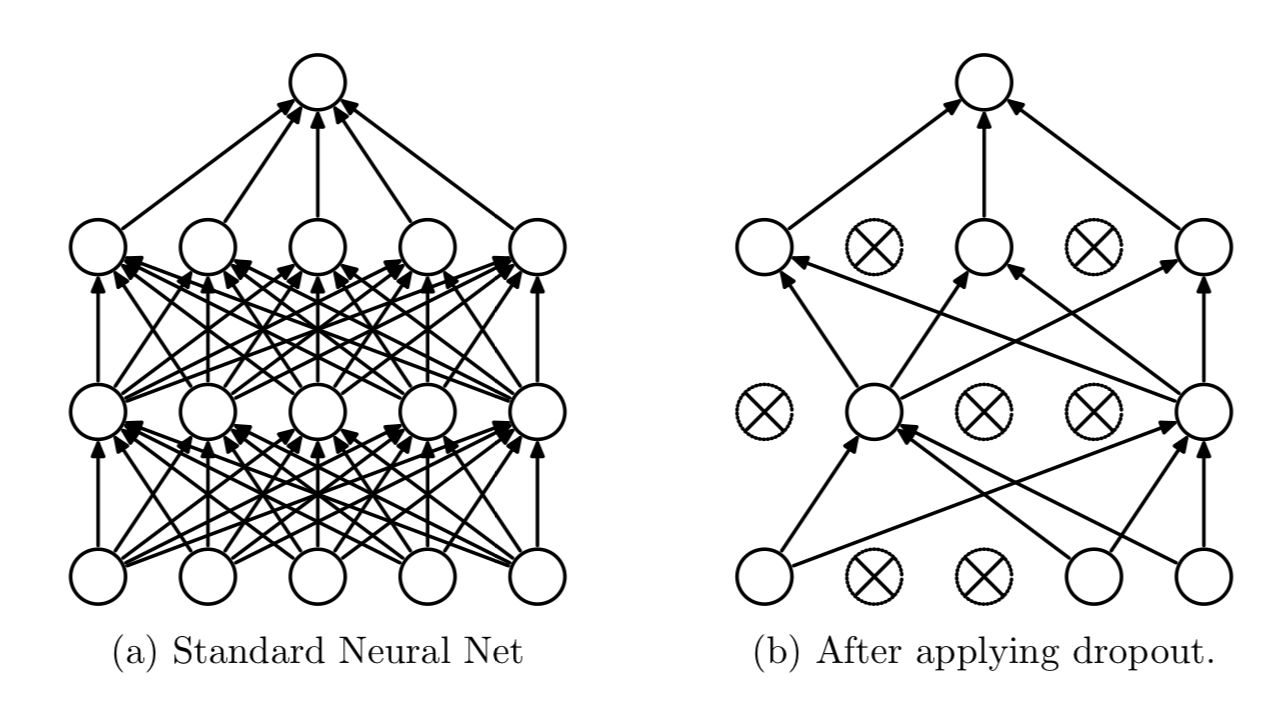
\includegraphics[scale=0.3]{images/dropout}}
\only<2>{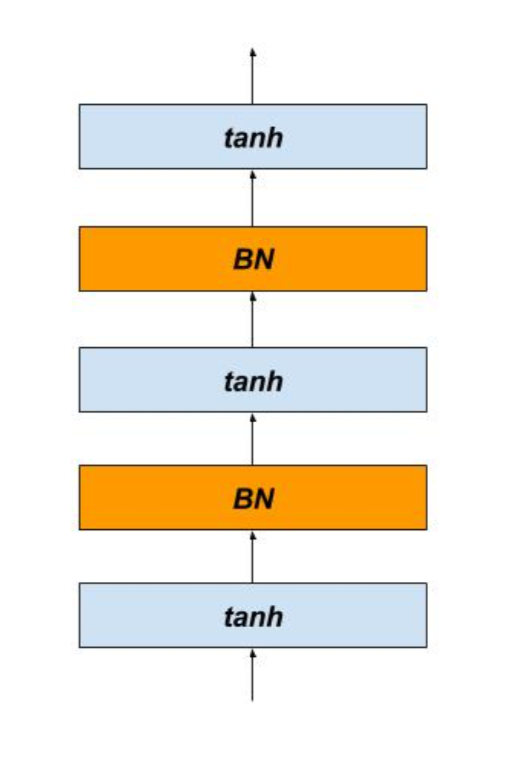
\includegraphics[scale=0.3]{images/batch_norm}}
\end{figure}
\end{overlayarea}
\end{columns}
\end{minipage}
\begin{minipage}[t][0.4\textheight][t]{\textwidth}
\begin{overlayarea}{\textwidth}{\textheight}
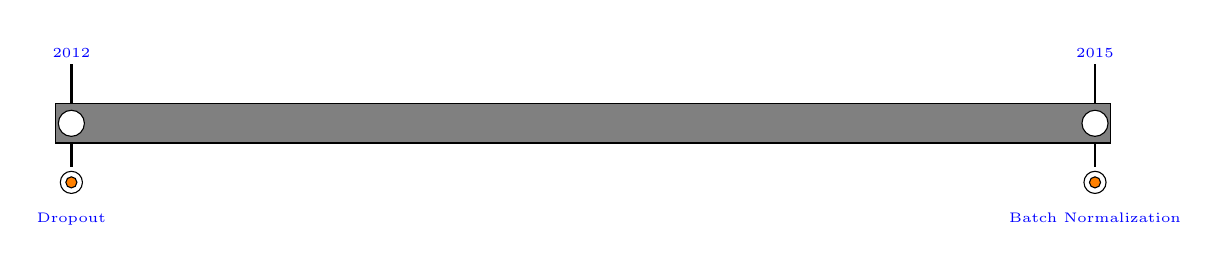
\begin{tikzpicture}[datemarker/.style={circle, draw=black,fill=white},textlabel/.style={anchor=center,text height=1.7ex,text depth=.25ex}]
\tikzset{every node/.style={font=\tiny, color=blue}}\draw[fill=gray](-0.2,0) rectangle (13.2,0.5) node[white, below]{};
\onslide<1->{\node at (0.0, 0.25) [datemarker] {};}
\onslide<1->{\draw [line width=1pt] (0.0, 0.5) to (0.0, 1.0);}
\onslide<1->{\draw (0.0, 1.2) node [textlabel]{2012};}
\onslide<1->{\draw [fill=orange](0.0, -0.5) circle (2pt){};}
\onslide<1->{\draw(0.0, -0.5) circle (4pt){};}
\onslide<1->{\draw [line width=1pt] (0.0, 0) to (0.0, -0.3);}
\onslide<1->{\draw (0.0,-0.9) node [textlabel] {Dropout};}
\onslide<2->{\node at (13.0, 0.25) [datemarker] {};}
\onslide<2->{\draw [line width=1pt] (13.0, 0.5) to (13.0, 1.0);}
\onslide<2->{\draw (13.0, 1.2) node [textlabel]{2015};}
\onslide<2->{\draw [fill=orange](13.0, -0.5) circle (2pt){};}
\onslide<2->{\draw(13.0, -0.5) circle (4pt){};}
\onslide<2->{\draw [line width=1pt] (13.0, 0) to (13.0, -0.3);}
\onslide<2->{\draw (13.0,-0.9) node [textlabel] {Batch Normalization};}
\end{tikzpicture}
\end{overlayarea}
\end{minipage}



\makeatother
%	\author{Mitesh M. Khapra}
	\title{Module 6}
	\subtitle{The Curious Case of Sequences}
		\author{}
		\institute{}
	\date{}
%\institute{Department of Computer Science and Engineering\\ Indian Institute of Technology Madras}
%\titlegraphic{
\includegraphics[height=1cm,width=2cm]{images/iitm_logo.png}}
%\titlegraphicii{\includegraphics[height=1cm,width=2cm]{logo2}}

\begin{frame}
	\myheading{Chapter 6: The Curious Case of Sequences}
\end{frame}

\begin{frame}
\begin{minipage}[t][0.6\textheight][t]{\textwidth}
\begin{columns}
\column{0.5\textwidth}


\begin{overlayarea}{\textwidth}{\textheight}
\justify
\only<1>{\myheading{ Sequences}}
\only<2>{\myheading{Hopfield Network}}
\only<3>{\myheading{Jordan Network}}
\only<4>{\myheading{Elman Network}}
\only<5>{\myheading{Drawbacks of RNNs}}
\only<6>{\myheading{Long Short Term Memory}}
\only<7>{\myheading{Sequence To Sequence Learning}}
\only<8>{\myheading{RL for Attention}}
\only<1>{\begin{itemize} \item They are everywhere \item Time series, speech, music, text, video \item Each unit in the sequence interacts with other units \item Need models to capture this interaction \end{itemize}}
\only<2>{Content-addressable memory systems for storing and retrieving patterns \cite{Hopfield:82}}
\only<3>{The output state of each time step is fed to the next time step thereby allowing interactions between time steps in the sequence}
\only<4>{The hidden state of each time step is fed to the next time step thereby allowing interactions between time steps in the sequence}
\only<5>{Hochreiter et. al. and Bengio et. al. showed the difficulty in training RNNs (the problem of exploding and vanishing gradients)}
\only<6>{Showed that LSTMs can solve complex long time lag tasks that could never be solved before}
\only<7>{\begin{itemize} \item Initial success in using RNNs/LSTMs for large scale Sequence To Sequence Learning Problems \item Introduction of Attention which inspired a lot of research over the next two years \end{itemize}}
\only<8>{Schmidhuber \& Huber proposed RNNs that use reinforcement learning to decide where to look}
\end{overlayarea}
\column{0.5\textwidth}
\begin{overlayarea}{\textwidth}{\textheight}
\begin{figure}

\only<2>{\includegraphics[scale=0.25]{"images/RNN/1982_1"}}
\only<3>{\includegraphics[scale=0.3]{"images/RNN/1986"}}
\only<4>{\includegraphics[scale=0.3]{"images/RNN/1990"}}
\only<6>{\includegraphics[scale=0.3]{"images/RNN/1997"}}
\only<7>{\includegraphics[scale=0.1]{"images/RNN/2014"}}
\end{figure}
\end{overlayarea}
\end{columns}
\end{minipage}
\begin{minipage}[t][0.4\textheight][t]{\textwidth}
\begin{overlayarea}{\textwidth}{\textheight}
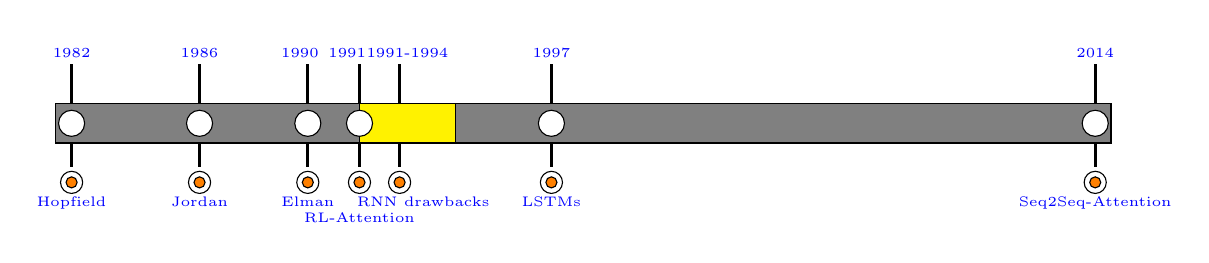
\begin{tikzpicture}[datemarker/.style={circle, draw=black,fill=white},textlabel/.style={anchor=center,text height=1.7ex,text depth=.25ex}] 
\tikzset{every node/.style={font=\tiny, color=blue}}\draw[fill=gray](-0.2,0) rectangle (13.2,0.5) node[white, below]{}; 

\onslide<2->{\node at (0.0, 0.25) [datemarker] {};}
\onslide<2->{\draw [line width=1pt] (0.0, 0.5) to (0.0, 1.0);} 
\onslide<2->{\draw (0.0, 1.2) node [textlabel] {1982 };}
\onslide<2->{\draw [fill=orange](0.0, -0.5) circle (2pt){};}
\onslide<2->{\draw (0.0, -0.5) circle (4pt){};}
\onslide<2->{\draw [line width=1pt] (0.0, 0) to (0.0, -0.3);}
\onslide<2->{\draw (0.0,-0.7) node [textlabel] {Hopfield};}

\onslide<3->{\node at (1.625, 0.25) [datemarker] {};}
\onslide<3->{\draw [line width=1pt] (1.625, 0.5) to (1.625, 1.0);} 
\onslide<3->{\draw (1.625, 1.2) node [textlabel] {1986 };}
\onslide<3->{\draw [fill=orange](1.625, -0.5) circle (2pt){};}
\onslide<3->{\draw (1.625, -0.5) circle (4pt){};}
\onslide<3->{\draw [line width=1pt] (1.625, 0) to (1.625, -0.3);}
\onslide<3->{\draw (1.625,-0.7) node [textlabel] {Jordan};}

\onslide<4->{\node at (3, 0.25) [datemarker] {};}
\onslide<4->{\draw [line width=1pt] (3, 0.5) to (3, 1.0);} 
\onslide<4->{\draw (2.9, 1.2) node [textlabel] {1990 };}
\onslide<4->{\draw [fill=orange](3, -0.5) circle (2pt){};}
\onslide<4->{\draw (3, -0.5) circle (4pt){};}
\onslide<4->{\draw [line width=1pt] (3, 0) to (3, -0.3);}
\onslide<4->{\draw (3,-0.7) node [textlabel] {Elman};}

\onslide<5->{\draw[fill=yellow](3.65625,0) rectangle (4.875,0.5){};}
\onslide<5->{\draw [line width=1pt] (4.165625, 0.5) to (4.165625, 1.0);} 
\onslide<5->{\draw (4.265625, 1.2) node [textlabel] {1991-1994 };}
\onslide<5->{\draw [fill=orange](4.165625, -0.5) circle (2pt){};}
\onslide<5->{\draw (4.165625, -0.5) circle (4pt){};}
\onslide<5->{\draw [line width=1pt] (4.165625, 0) to (4.165625, -0.3);}
\onslide<5->{\draw (4.465625,-0.7) node [textlabel] {RNN drawbacks};}


\onslide<6->{\node at (6.09375, 0.25) [datemarker] {};}
\onslide<6->{\draw [line width=1pt] (6.09375, 0.5) to (6.09375, 1.0);} 
\onslide<6->{\draw (6.09375, 1.2) node [textlabel] {1997 };}
\onslide<6->{\draw [fill=orange](6.09375, -0.5) circle (2pt){};}
\onslide<6->{\draw (6.09375, -0.5) circle (4pt){};}
\onslide<6->{\draw [line width=1pt] (6.09375, 0) to (6.09375, -0.3);}
\onslide<6->{\draw (6.09375,-0.7) node [textlabel] {LSTMs};}

\onslide<7->{\node at (13.0, 0.25) [datemarker] {};}
\onslide<7->{\draw [line width=1pt] (13.0, 0.5) to (13.0, 1.0);} 
\onslide<7->{\draw (13.0, 1.2) node [textlabel] {2014 };}
\onslide<7->{\draw [fill=orange](13.0, -0.5) circle (2pt){};}
\onslide<7->{\draw (13.0, -0.5) circle (4pt){};}
\onslide<7->{\draw [line width=1pt] (13.0, 0) to (13.0, -0.3);}
\onslide<7->{\draw (13.0,-0.7) node [textlabel] {Seq2Seq-Attention};}

\onslide<8->{\node at (3.65625, 0.25) [datemarker] {};}
\onslide<8->{\draw [line width=1pt] (3.65625, 0.5) to (3.65625, 1.0);} 
\onslide<8->{\draw (3.5, 1.2) node [textlabel] {1991 };}
\onslide<8->{\draw [fill=orange](3.65625, -0.5) circle (2pt){};}
\onslide<8->{\draw (3.65625, -0.5) circle (4pt){};}
\onslide<8->{\draw [line width=1pt] (3.65625, 0) to (3.65625, -0.3);}
\onslide<8->{\draw (3.65625,-0.9) node [textlabel] {RL-Attention};}
\end{tikzpicture}
\end{overlayarea}
\end{minipage}
\end{frame}

%	\author{Mitesh M. Khapra}
	\title{Module 7}
	\subtitle{Beating humans at their own game (literally)}
		\author{}
		\institute{}
	\date{}
%\institute{Department of Computer Science and Engineering\\ Indian Institute of Technology Madras}
%\titlegraphic{\includegraphics[height=1cm,width=2cm]{images/iitm_logo.png}}
%\titlegraphicii{\includegraphics[height=1cm,width=2cm]{logo2}}

\begin{frame}
	\myheading{Beating humans at their own game (literally)}
\end{frame}

\begin{frame}
\begin{minipage}[t][0.6\textheight][t]{\textwidth}
\begin{columns}
\column{0.5\textwidth}
\begin{overlayarea}{\textwidth}{\textheight}
\justify
\only<1>{\myheading{Playing Atari Games}}
\only<2>{\myheading{Let's GO}}
\only<3>{\myheading{Taking a shot at Poker}}
\only<4>{\myheading{Defense of the Ancients}}
\only<1>{\begin{itemize}
		\item{
		Human-level control through deep reinforcement learning for playing Atari Games}
		\end{itemize}}
\only<2>{\begin{itemize}
		\item{Alpha Go Zero - Best Go player ever, surpassing human players}
		\item{GO is more complex than chess because of number of possible moves.}
		\item{No brute force backtracking unlike previous chess agents }
		\end{itemize}}
\only<3>{\textbf{DeepStack} defeated 11 professional poker players with only one outside the margin of statistical significance.}
\only<4>{\begin{itemize}
\item{Widely popular game, with complex strategies, large visual space}
\item{Bot was undefeated against many top professional players . }
\end{itemize}}
\end{overlayarea}
\column{0.5\textwidth}
\begin{overlayarea}{\textwidth}{\textheight}
\begin{figure}
\centering
\only<1>{\includegraphics[scale=0.2]{images/atari}}
\only<2>{\includegraphics[scale=0.2]{images/alphago}}
\only<3>{\includegraphics[scale=0.15]{images/poker}}
\only<4>{\includegraphics[scale=0.15]{images/dota}}
\end{figure}
\end{overlayarea}
\end{columns}
\end{minipage}
\begin{minipage}[t][0.4\textheight][t]{\textwidth}
\begin{overlayarea}{\textwidth}{\textheight}
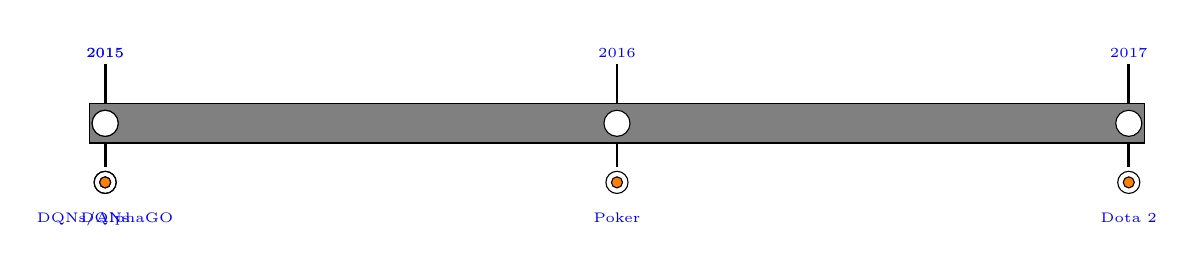
\begin{tikzpicture}[datemarker/.style={circle, draw=black,fill=white},textlabel/.style={anchor=center,text height=1.7ex,text depth=.25ex}]
\tikzset{every node/.style={font=\tiny, color=blue}}\draw[fill=gray](-0.2,0) rectangle (13.2,0.5) node[white, below]{};
\onslide<1->{\node at (0.0, 0.25) [datemarker] {};}
\onslide<1->{\draw [line width=1pt] (0.0, 0.5) to (0.0, 1.0);}
\onslide<1->{\draw (0.0, 1.2) node [textlabel]{2015};}
\onslide<1->{\draw [fill=orange](0.0, -0.5) circle (2pt){};}
\onslide<1->{\draw(0.0, -0.5) circle (4pt){};}
\onslide<1->{\draw [line width=1pt] (0.0, 0) to (0.0, -0.3);}
\onslide<1>{\draw (0.0,-0.9) node [textlabel] {DQNs};}
\onslide<2->{\node at (0.0, 0.25) [datemarker] {};}
\onslide<2->{\draw [line width=1pt] (0.0, 0.5) to (0.0, 1.0);}
\onslide<2->{\draw (0.0, 1.2) node [textlabel]{2015};}
\onslide<2->{\draw [fill=orange](0.0, -0.5) circle (2pt){};}
\onslide<2->{\draw(0.0, -0.5) circle (4pt){};}
\onslide<2->{\draw [line width=1pt] (0.0, 0) to (0.0, -0.3);}
\onslide<2->{\draw (0.0,-0.9) node [textlabel] {DQNs/AlphaGO};}
\onslide<3->{\node at (6.5, 0.25) [datemarker] {};}
\onslide<3->{\draw [line width=1pt] (6.5, 0.5) to (6.5, 1.0);}
\onslide<3->{\draw (6.5, 1.2) node [textlabel]{2016};}
\onslide<3->{\draw [fill=orange](6.5, -0.5) circle (2pt){};}
\onslide<3->{\draw(6.5, -0.5) circle (4pt){};}
\onslide<3->{\draw [line width=1pt] (6.5, 0) to (6.5, -0.3);}
\onslide<3->{\draw (6.5,-0.9) node [textlabel] {Poker};}
\onslide<4->{\node at (13.0, 0.25) [datemarker] {};}
\onslide<4->{\draw [line width=1pt] (13.0, 0.5) to (13.0, 1.0);}
\onslide<4->{\draw (13.0, 1.2) node [textlabel]{2017};}
\onslide<4->{\draw [fill=orange](13.0, -0.5) circle (2pt){};}
\onslide<4->{\draw(13.0, -0.5) circle (4pt){};}
\onslide<4->{\draw [line width=1pt] (13.0, 0) to (13.0, -0.3);}
\onslide<4->{\draw (13.0,-0.9) node [textlabel] {Dota 2};}
\end{tikzpicture}
\end{overlayarea}
\end{minipage}
\end{frame}


\makeatother
% \author{Mitesh M. Khapra}
  \title{Module 8}
  \subtitle{The Madness (2013-)}
    \author{}
    \institute{}
  \date{}
%\institute{Department of Computer Science and Engineering\\ Indian Institute of Technology Madras}
%\titlegraphic{\includegraphics[height=1cm,width=2cm]{images/iitm_logo.png}}
%\titlegraphicii{\includegraphics[height=1cm,width=2cm]{logo2}}

\begin{frame}
  \myheading{Chapter 8: The Madness (2013-)}
\end{frame}

\begin{frame}
\begin{columns}            
\begin{column}{0.6\textwidth}
\begin{overlayarea}{\textwidth}{\textheight}
\vspace{0.2in}
\hspace{1cm}\textbf{He sat on a \underline{chair}.}
\end{overlayarea}
\end{column}

\begin{column}{0.4\textwidth}
\begin{overlayarea}{\textwidth}{\textheight}

\begin{block}{Language Modeling}
\begin{itemize}
\item Mikolov et al. (2010) \cite{DBLP:conf/interspeech/MikolovKBCK10}
\item Li et al. (2015)  
\item Kiros et al. (2015) \cite{DBLP:conf/nips/KirosZSZUTF15}
\item Kim et al. (2015) \cite{DBLP:journals/corr/KimJSR15}
\end{itemize}
\end{block}
\end{overlayarea}
\end{column}

\end{columns}
\end{frame}

\begin{frame}
\begin{columns}            
\begin{column}{0.6\textwidth}
\begin{overlayarea}{\textwidth}{\textheight}
\vspace{0.2in}
\includegraphics[width=0.8\linewidth]{images/speechrecog}
\end{overlayarea}
\end{column}

\begin{column}{0.4\textwidth}
\begin{overlayarea}{\textwidth}{\textheight}

              \begin{block}{Speech Recognition}
                \begin{itemize}
                  \item Hinton et al. (2012) \cite{DBLP:journals/spm/X12a}
                  \item Graves et al. (2013) \cite{DBLP:conf/icassp/GravesMH13}
                  \item Chorowski et al. (2015) \cite{DBLP:conf/nips/ChorowskiBSCB15}
                  \item Sak et al. (2015) \cite{DBLP:conf/interspeech/SakSRB15}
                \end{itemize}
              \end{block}
\end{overlayarea}
\end{column}

\end{columns}
\end{frame}


\begin{frame}
\begin{columns}            
\begin{column}{0.6\textwidth}
\begin{overlayarea}{\textwidth}{\textheight}
\vspace{0.2in}
                \includegraphics[width=1\linewidth]{images/Mt}
\end{overlayarea}
\end{column}

\begin{column}{0.4\textwidth}
\begin{overlayarea}{\textwidth}{\textheight}

              \begin{block}{Machine Translation}

                \begin{itemize}
                  \item Kalchbrenner et al. (2013) \cite{DBLP:conf/emnlp/KalchbrennerB13}
                  \item Cho et al. (2014) \cite{DBLP:conf/emnlp/ChoMGBBSB14}
                  \item Bahdanau et al. (2015) \cite{DBLP:journals/corr/BahdanauCB14}
                  \item Jean et al. (2015) \cite{DBLP:conf/acl/JeanCMB15}
                  \item Gulcehre et al. (2015) \cite{DBLP:journals/corr/GulcehreFXCBLBS15}
                  \item Sutskever et al. (2014) \cite{DBLP:conf/nips/SutskeverVL14}
                  \item Luong et al. (2015) \cite{DBLP:conf/emnlp/LuongPM15}
                  \item Zheng et al. (2017) \cite{DBLP:conf/ijcai/ZhengCL17}
                  \item Cheng et al. (2016) \cite{DBLP:conf/ijcai/ChengYLSX17}
                  \item Chen et al. (2017) \cite{DBLP:conf/acl/ChenLCL17}
                  \item Firat et al. (2016) \cite{DBLP:conf/emnlp/FiratSAYC16}
                \end{itemize}
              \end{block}
\end{overlayarea}
\end{column}

\end{columns}
\end{frame}

\begin{frame}
\begin{columns}            
\begin{column}{0.6\textwidth}
\vspace{0.2in}
\begin{overlayarea}{\textwidth}{\textheight}
                \includegraphics[width=0.85\linewidth]{images/cm}
\end{overlayarea}
\end{column}

\begin{column}{0.4\textwidth}
\begin{overlayarea}{\textwidth}{\textheight}

              \begin{block}{Conversation Modeling}
                \begin{itemize}
                  \item Shang et al. (2015) \cite{DBLP:conf/acl/ShangLL15}
                  \item Vinyals et al. (2015) \cite{DBLP:journals/corr/VinyalsL15}
                  \item Lowe et al. (2015) \cite{DBLP:conf/sigdial/LowePSP15}
                  \item Dodge et al. (2015) \cite{DBLP:journals/corr/DodgeGZBCMSW15}
                  \item Weston et al. (2016) \cite{DBLP:journals/corr/WestonBCM15}
                  \item Serban et al. (2016) \cite{DBLP:journals/corr/SerbanSLCPCB16}
                  \item Bordes et al. (2017) \cite{DBLP:journals/corr/BordesW16}
                  \item He et al. (2017)
                  \item Serban et al. (2017) \cite{DBLP:journals/corr/abs-1709-02349}
                  \item Lewis et al. (2017) 
                \end{itemize}
              \end{block}
\end{overlayarea}
\end{column}

\end{columns}
\end{frame}

\begin{frame}
    \begin{columns}
    
        \begin{column}{0.6\textwidth}
        \vspace{0.2in}
        \begin{overlayarea}{\textwidth}{\textheight}
                        \includegraphics[width=1\linewidth]{images/qa2}
        \end{overlayarea}
        \end{column}
        
        \begin{column}{0.4\textwidth}
            \begin{overlayarea}{\textwidth}{\textheight}
                \begin{block}{Question Answering}
                    \begin{itemize}
                        \item Hermann et al. (2015) \cite{DBLP:conf/nips/HermannKGEKSB15} 
                        \item Chen et al. (2016) \cite{DBLP:conf/acl/ChenBM16}
                        \item Xiong et al. (2016) \cite{DBLP:journals/corr/XiongZS16}
                        \item Seo et al. (2016) \cite{DBLP:journals/corr/SeoKFH16}
                        \item Dhingra et al. (2017) \cite{DBLP:conf/acl/DhingraLYCS17}
                        \item Wang et al. (2017) \cite{DBLP:conf/acl/WangYWCZ17}
                        \item Hu et al. (2017) \cite{DBLP:journals/corr/HuPQ17}
                    \end{itemize}
                \end{block}
            \end{overlayarea}
        \end{column}
        
    \end{columns}
\end{frame}


\begin{frame}
    \begin{columns}            
        \begin{column}{0.5\textwidth}
            \vspace{0.2in}
            \begin{overlayarea}{\textwidth}{\textheight}
                            \includegraphics[width=1\linewidth]{images/or}
            \end{overlayarea}
        \end{column}
        
        \begin{column}{0.5\textwidth}
            \begin{overlayarea}{\textwidth}{\textheight}
                \vspace{-5mm}
                \begin{block}{Object Detection/Recognition}
                    \begin{itemize}
                    %   \item Segmenting Object candidates (Pinheiro et al., 2015) 
                    %   \item Scene Labeling (Byeon et al., 2015)
                    %   \item Object-class segmentation in Videos (Serban et al., 2015)
                    %   \item Zheng et al. (2015)
                    %   \item PVANET (Kim et al., 2016)
                      \item Semantic Segmentation (Long et al, 2015) \cite{DBLP:conf/cvpr/LongSD15}
                      \item Recurrent CNNs (Liang et al., 2015) \cite{DBLP:conf/cvpr/LiangH15}
                      \item Faster RCNN (Ren et al., 2015) \cite{DBLP:journals/pami/RenHG017}
                      \item Inside-Outside Net (Bell et al., 2015) \cite{DBLP:journals/corr/BellZBG15}
                      \item YOLO9000 (Redmon et al., 2016) \cite{DBLP:journals/corr/RedmonF16}
                      \item R-FCN (Dai et al., 2016) \cite{DBLP:conf/nips/DaiLHS16}
                      %\item Deformable CNN + R-FCN (Dai et al., 2017) \cite{DBLP:journals/corr/DaiQXLZHW17}
                      \item Mask R-CNN (He at al., 2017) \cite{DBLP:conf/iccv/HeGDG17}
                      \item Video Object segmentation (Caelles et al., 2017) \cite{DBLP:conf/cvpr/CaellesMPLCG17}
                    \end{itemize}
                \end{block}
            \end{overlayarea}
        \end{column}
    \end{columns}
\end{frame}



\begin{frame}
\begin{columns}            
\begin{column}{0.6\textwidth}
\vspace{0.2in}
\begin{overlayarea}{\textwidth}{\textheight}
                \includegraphics[width=\linewidth]{images/vt}
\end{overlayarea}
\end{column}

\begin{column}{0.4\textwidth}
\begin{overlayarea}{\textwidth}{\textheight}

              \begin{block}{Visual Tracking
                }
                \begin{itemize}
                  \item Zhang et al. (2017) 
                  \item Choi et al. (2017) \cite{DBLP:journals/corr/ChoiKL17}
                  \item Yun et al. (2017) \cite{DBLP:conf/cvpr/YunCYYC17}
                  \item Luo et al. (2017)
                  \item Alahi et al. (2017) \cite{DBLP:journals/corr/SadeghianAS17}
                  \item Van et al. (2016)
                \end{itemize}
              \end{block}
\end{overlayarea}
\end{column}

\end{columns}
\end{frame}

\begin{frame}
\begin{columns}            
\begin{column}{0.6\textwidth}
\vspace{0.2in}
\begin{overlayarea}{\textwidth}{\textheight}
                \includegraphics[width=1\linewidth]{images/ic}
\end{overlayarea}
\end{column}

\begin{column}{0.4\textwidth}
\begin{overlayarea}{\textwidth}{\textheight}

              \begin{block}{Image Captioning
                }
                \begin{itemize}
                  \item Mao et al. (2014) \cite{DBLP:journals/corr/MaoXYWY14a}
                  \item Mao at al. (2015) \cite{Mao_2015_ICCV}
                  \item Kiros et al. (2015) \cite{DBLP:journals/corr/KirosSZ14}
                  \item Donahue et al. (2015) \cite{DBLP:conf/cvpr/DonahueHGRVDS15}
                  \item Vinyals et al. (2015) \cite{DBLP:conf/cvpr/VinyalsTBE15}
                  \item Karpathy et al. (2015) \cite{DBLP:conf/cvpr/KarpathyL15}
                  \item Fang et al. (2015) \cite{DBLP:conf/cvpr/FangGISDDGHMPZZ15}
                  \item Chen et al. (2015) \cite{DBLP:journals/corr/ChenWCGXN15}
                \end{itemize}
              \end{block}
\end{overlayarea}
\end{column}

\end{columns}
\end{frame}

\begin{frame}
\begin{columns}            
\begin{column}{0.6\textwidth}
\vspace{0.2in}
\begin{overlayarea}{\textwidth}{\textheight}
                \includegraphics[width=1\linewidth]{images/vc}
\end{overlayarea}
\end{column}

\begin{column}{0.4\textwidth}
\begin{overlayarea}{\textwidth}{\textheight}

              \begin{block}{Video Captioning
                }
                \begin{itemize}
                  \item Donahue et al. (2014) \cite{DBLP:journals/corr/DonahueHGRVSD14}
                  \item Venugopalan at al. (2014) \cite{DBLP:conf/naacl/VenugopalanXDRM15}
                  \item Pan et al. (2015) \cite{DBLP:journals/corr/PanMYLR15}
                  \item Yao et al. (2015) \cite{DBLP:conf/iccv/YaoTCBPLC15}
                  \item Rohrbach et al. (2015) \cite{DBLP:conf/dagm/RohrbachRQFPS14}
                  \item Zhu et al. (2015) \cite{DBLP:journals/corr/ZhuXYH15}
                  \item Cho et al. (2015) \cite{DBLP:conf/emnlp/ChoMGBBSB14}
                  \item S. Sha 2017
                \end{itemize}
              \end{block}
\end{overlayarea}
\end{column}

\end{columns}
\end{frame}


\begin{frame}
\begin{columns}            
\begin{column}{0.6\textwidth}
\vspace{0.2in}
\begin{overlayarea}{\textwidth}{\textheight}
                \includegraphics[width=1\linewidth]{images/visualQA.png}
\end{overlayarea}
\end{column}

\begin{column}{0.4\textwidth}
\begin{overlayarea}{\textwidth}{\textheight}

              \begin{block}{Visual Question Answering
                }
                \begin{itemize}
                  \item Santoro et al. (2017) \cite{DBLP:conf/nips/SantoroRBMPBL17} 
                  \item Hu at al. (2017) \cite{DBLP:conf/iccv/HuARDS17}
                  \item Johnson et al. (2017) \cite{DBLP:conf/cvpr/JohnsonHMFZG17}
                  \item Ben-younes et al. (2017) \cite{DBLP:conf/iccv/Ben-younesCCT17}
                  \item Malinowski et al. (2017) \cite{DBLP:conf/iccv/MalinowskiRF15}
                  \item Nam et al. (2016)
                  \item Kazemi et al. (2016) \cite{DBLP:journals/corr/KazemiE17}
                \end{itemize}
              \end{block}
\end{overlayarea}
\end{column}

\end{columns}
\end{frame}


\begin{frame}
\begin{columns}            
\begin{column}{0.6\textwidth}
\vspace{0.2in}
\begin{overlayarea}{\textwidth}{\textheight}
                \includegraphics[scale=0.25]{images/fill-in-blank.png}\\
                \includegraphics[scale=0.3]{images/open-end-video-QA.png}\\
\end{overlayarea}
\end{column}

\begin{column}{0.4\textwidth}
\begin{overlayarea}{\textwidth}{\textheight}

              \begin{block}{Video Question Answering
                }
                \begin{itemize}
                    \item Tapaswi et. al. 2016 \cite{DBLP:conf/cvpr/TapaswiZSTUF16}
                    \item Zeng et. al. 2016 \cite{DBLP:journals/corr/ZengCCLNS16}
                    \item Maharaj et. al. 2017 \cite{DBLP:conf/cvpr/MaharajBRCP17}
                    \item Zhao et. al. 2017 \cite{DBLP:conf/ijcai/ZhaoYCHZ17}
                    \item Yu Youngjae et. al. 2017 \cite{DBLP:conf/cvpr/YuKCK17}
                    \item Xue Hongyang et. al. 2017 \cite{DBLP:journals/corr/XueZC17}
                    \item Mazaheri et. al. 2017 \cite{DBLP:journals/corr/MazaheriZS16}
                    \end{itemize}
              \end{block}
\end{overlayarea}
\end{column}

\end{columns}
\end{frame}

\begin{frame}
\begin{columns}            
\begin{column}{0.6\textwidth}
\vspace{0.2in}
\begin{overlayarea}{\textwidth}{\textheight}
                \includegraphics[width=1\textwidth]{images/video-abstraction.png}\\
            
\end{overlayarea}
\end{column}

\begin{column}{0.4\textwidth}
\begin{overlayarea}{\textwidth}{\textheight}
              \begin{block}{Video Summarization}
                \begin{itemize}
                    \item Chheng 2007 \cite{Chheng_videosummarization}
                    \item Ajmal 2012 \cite{DBLP:conf/iccvg/AjmalASAS12}
                    \item Zhang Ke 2016 \cite{DBLP:conf/eccv/ZhangCSG16}
                    \item Zhong Ji 2017 \cite{DBLP:journals/corr/abs-1708-09545}
                    \item Panda 2017 \cite{DBLP:journals/tip/PandaMR17}
                    
                    \end{itemize}
              \end{block}
\end{overlayarea}
\end{column}

\end{columns}
\end{frame}

\begin{frame}
\begin{columns}            
\begin{column}{0.6\textwidth}
\vspace{0.2in}
\begin{overlayarea}{\textwidth}{\textheight}
                \includegraphics[scale=0.5]{images/va}
\end{overlayarea}
\end{column}

\begin{column}{0.4\textwidth}
\begin{overlayarea}{\textwidth}{\textheight}

              \begin{block}{Generating Authentic Photos}
                \begin{itemize}
                  \item Variational Autoencoders (Kingma et. al., 2013) \cite{DBLP:journals/corr/KingmaW13}
                  \item Generative Adversarial Networks (Goodfellow et. al., 2014) \cite{DBLP:conf/nips/GoodfellowPMXWOCB14}
                  \item Plug \& Play generative nets (Nguyen et al., 2016) \cite{DBLP:journals/corr/NguyenYBDC16}
                  \item Progressive Growing of GANs (Karras et al., 2017) \cite{DBLP:journals/corr/abs-1710-10196}
                \end{itemize}
              \end{block}
\end{overlayarea}
\end{column}
\end{columns}
\end{frame}

\begin{frame}
\begin{columns}            
\begin{column}{0.6\textwidth}
\vspace{0.2in}
\begin{overlayarea}{\textwidth}{\textheight}
                \includegraphics[width=1\linewidth]{images/wave}
\end{overlayarea}
\end{column}

\begin{column}{0.4\textwidth}
\begin{overlayarea}{\textwidth}{\textheight}

              \begin{block}{Generating Raw Audio}
                \begin{itemize}
                  \item Wavenets (Oord et. al., 2016) \cite{45774}
                \end{itemize}
              \end{block}
\end{overlayarea}
\end{column}
\end{columns}
\end{frame}

\begin{frame}
\begin{columns}            
\begin{column}{0.6\textwidth}
\vspace{0.2in}
\begin{overlayarea}{\textwidth}{\textheight}
                \includegraphics[width=1\linewidth]{images/pixel_rnn}
                \end{overlayarea}
\end{column}
\begin{column}{0.4\textwidth}
\begin{overlayarea}{\textwidth}{\textheight}
              \begin{block}{Pixel RNNs}
                \begin{itemize}
                  \item (Oord et al., 2016) \cite{pixelRNN}
                  \item (Oord et al., 2016) \cite{pixelcnn}
                  \item (Salimans et al., 2017) \cite{salimans2017pixelcnn++}
                \end{itemize}
              \end{block}
\end{overlayarea}
\end{column}
\end{columns}
\end{frame}


	\makeatother
	%	\author{Mitesh M. Khapra}
		\title{Module 9}
		\subtitle{(Need for) Sanity}
			\author{}
			\institute{}
		\date{}
	%\institute{Department of Computer Science and Engineering\\ Indian Institute of Technology Madras}
	%\titlegraphic{\includegraphics[height=1cm,width=2cm]{images/iitm_logo.png}}
	%\titlegraphicii{\includegraphics[height=1cm,width=2cm]{logo2}}
	\renewcommand{\thefootnote}{\roman{footnote}} 
	\begin{frame}
		\myheading{Chapter 9: (Need for) Sanity}
	\end{frame}
	\begin{frame}
	\begin{columns}
	\column{0.55\textwidth}
	\begin{overlayarea}{\textwidth}{\textheight}
	\footnotesize{
	\justify
	\myheading{The Paradox of Deep Learning} 
	Why does deep learning work so well despite 
	\begin{itemize} 
	\item<2-> {high capacity (susceptible to overfitting)}
	\item<3-> {numerical instability (vanishing/exploding gradients)}
	\item<4-> {sharp minima (leading to overfitting)}
	\item<5-> {non-robustness (see figure)}
	\end{itemize}
	~\\
	\only<6->{No clear answers yet but ...}
	\begin{itemize} \justifying
	\item<7->{Slowly but steadily there is increasing emphasis on explainability and theoretical justifications! \footnote[1]{https://arxiv.org/pdf/1710.05468.pdf}}
	\item<8->{ Hopefully this will bring sanity to the proceedings !}
	\end{itemize}}
	\end{overlayarea}
	\column{0.45\textwidth}
	\begin{overlayarea}{\textwidth}{\textheight}
	\begin{figure}
	\centering
	\vspace{0.2in}
	\only<1->{\includegraphics[scale=0.4]{"images/adversarial_img_1"}}
	\end{figure}
	\end{overlayarea}
	\end{columns}
	\end{frame}


\begin{frame}
    \centering
    \small{\url{https://github.com/kjw0612/awesome-rnn}}
\end{frame}

\begin{frame}
    \begin{figure}[ht]
        \centering
        \fcolorbox{black}{gray}{\includegraphics[width=1\linewidth]{images/Deep_learning_MarketMap_sept2016_featured}}
%      \label{fig:startups}
%      \caption*{The Deep Learning Market Map}
      
    \end{figure}
    \footnotetext[1]{Source: https://www.cbinsights.com/blog/deep-learning-ai-startups-market-map-company-list/}
\end{frame}
  


\begin{frame}[allowframebreaks]{References}
\nocite{*}
\tiny
\bibliographystyle{unsrt}
\bibliography{ref}
    

\end{frame}
\end{document}
